\documentclass[11pt,
			   %10pt, 
               %hyperref={colorlinks},
               aspectratio=169,
               hyperref={colorlinks}
               ]{beamer}
\usetheme{Singapore}
\usecolortheme[snowy, cautious]{owl}

% Remove headline and navigation in the header
%\setbeamertemplate{headline}{}
%\setbeamertemplate{navigation symbols}{}

% navigation symbol
\usenavigationsymbolstemplate{}

\usepackage[utf8]{inputenc}
\usepackage[T1]{fontenc}
\usepackage[american]{babel}
\usepackage{graphicx}
\usepackage{hyperref}
\hypersetup{
    colorlinks=true,
    urlcolor=[rgb]{0,0,0.61},
    linkcolor=[rgb]{0,0,0.61}}
\definecolor{magenta}{RGB}{255, 0, 255}
     
\usepackage[natbib=true,style=authoryear,backend=bibtex,useprefix=true]{biblatex}

%\setbeamercolor*{bibliography entry title}{fg=black}
%\setbeamercolor*{bibliography entry location}{fg=black}
%\setbeamercolor*{bibliography entry note}{fg=black}
\definecolor{OwlGreen}{RGB}{51,0,102} % easier to see
\setbeamertemplate{bibliography item}{}
\setbeamerfont{caption}{size=\footnotesize}
\setbeamertemplate{frametitle continuation}{}
\setcounter{tocdepth}{2}
\renewcommand*{\bibfont}{\scriptsize}
\addbibresource{lecture_7.bib}

\renewcommand*{\thefootnote}{\fnsymbol{footnote}}



\setbeamertemplate{footline}{%
    \raisebox{5pt}{\makebox{\hfill\makebox[20pt]{\color{gray}
          \scriptsize\insertframenumber}}}\hspace*{5pt}}

          
\author{Patrick Hall}
\title{Responsible Machine Learning}
\subtitle{Lecture 7: Risk Mitigation Proposals for Language Models}
\institute{The George Washington University}
\date{\today}


\begin{document}
	
	\maketitle
	
	\begin{frame}{Contents\footnote{\tiny{WARNING: This presentation contains model outputs which are potentially offensive and disturbing in nature.}}}

	\begin{columns}[onlytextwidth]
		\column{0.5\textwidth}
		\tableofcontents[sections = 1-8]
		\column{0.5\textwidth}
		\tableofcontents[sections = 9-17]
	\end{columns}

	\end{frame}


	%-------------------------------------------------------------------------------
	\section{Technical Primer}
	%-------------------------------------------------------------------------------
		\subsection*{} % for slide tracking
		
		\begin{frame}
			\frametitle{Term Embedding (like \texttt{Word2Vec}, \cite{NIPS2013_9aa42b31})}
			\centering
			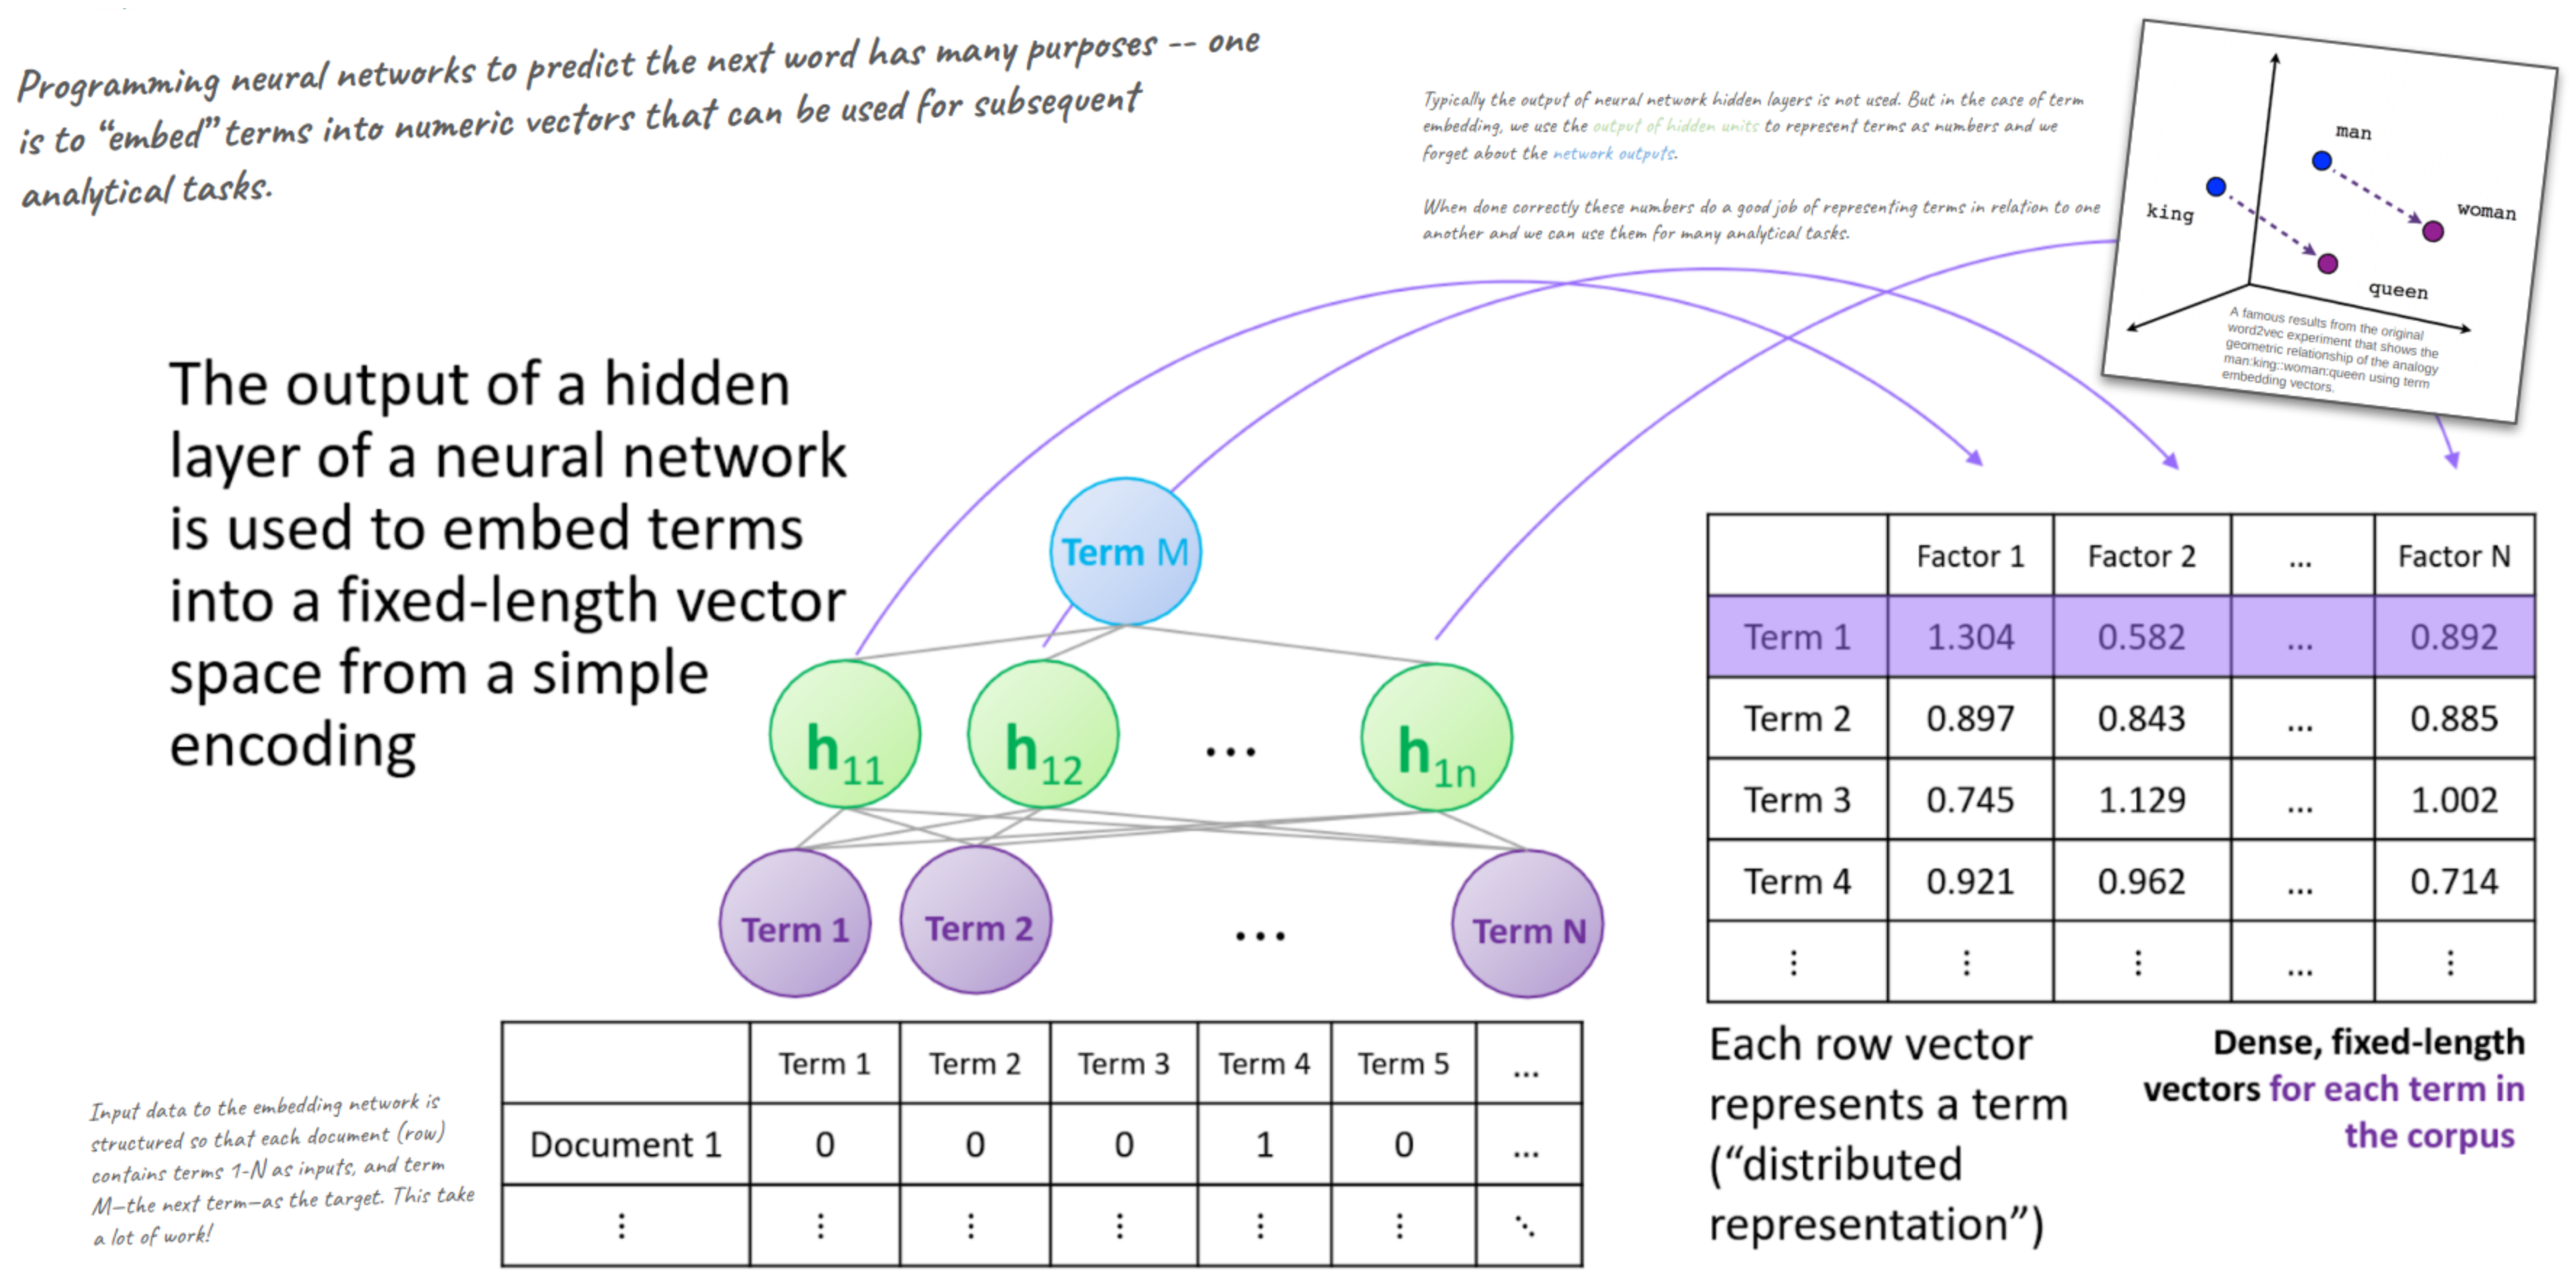
\includegraphics[height=200pt]{../img/embed.png}
		\end{frame}
		
		\begin{frame}
			\frametitle{\small{Sequence-to-sequence Learning with Recurrent Neural Networks\\ (RNNs, \cite{cho2014learning})}}
			\centering
			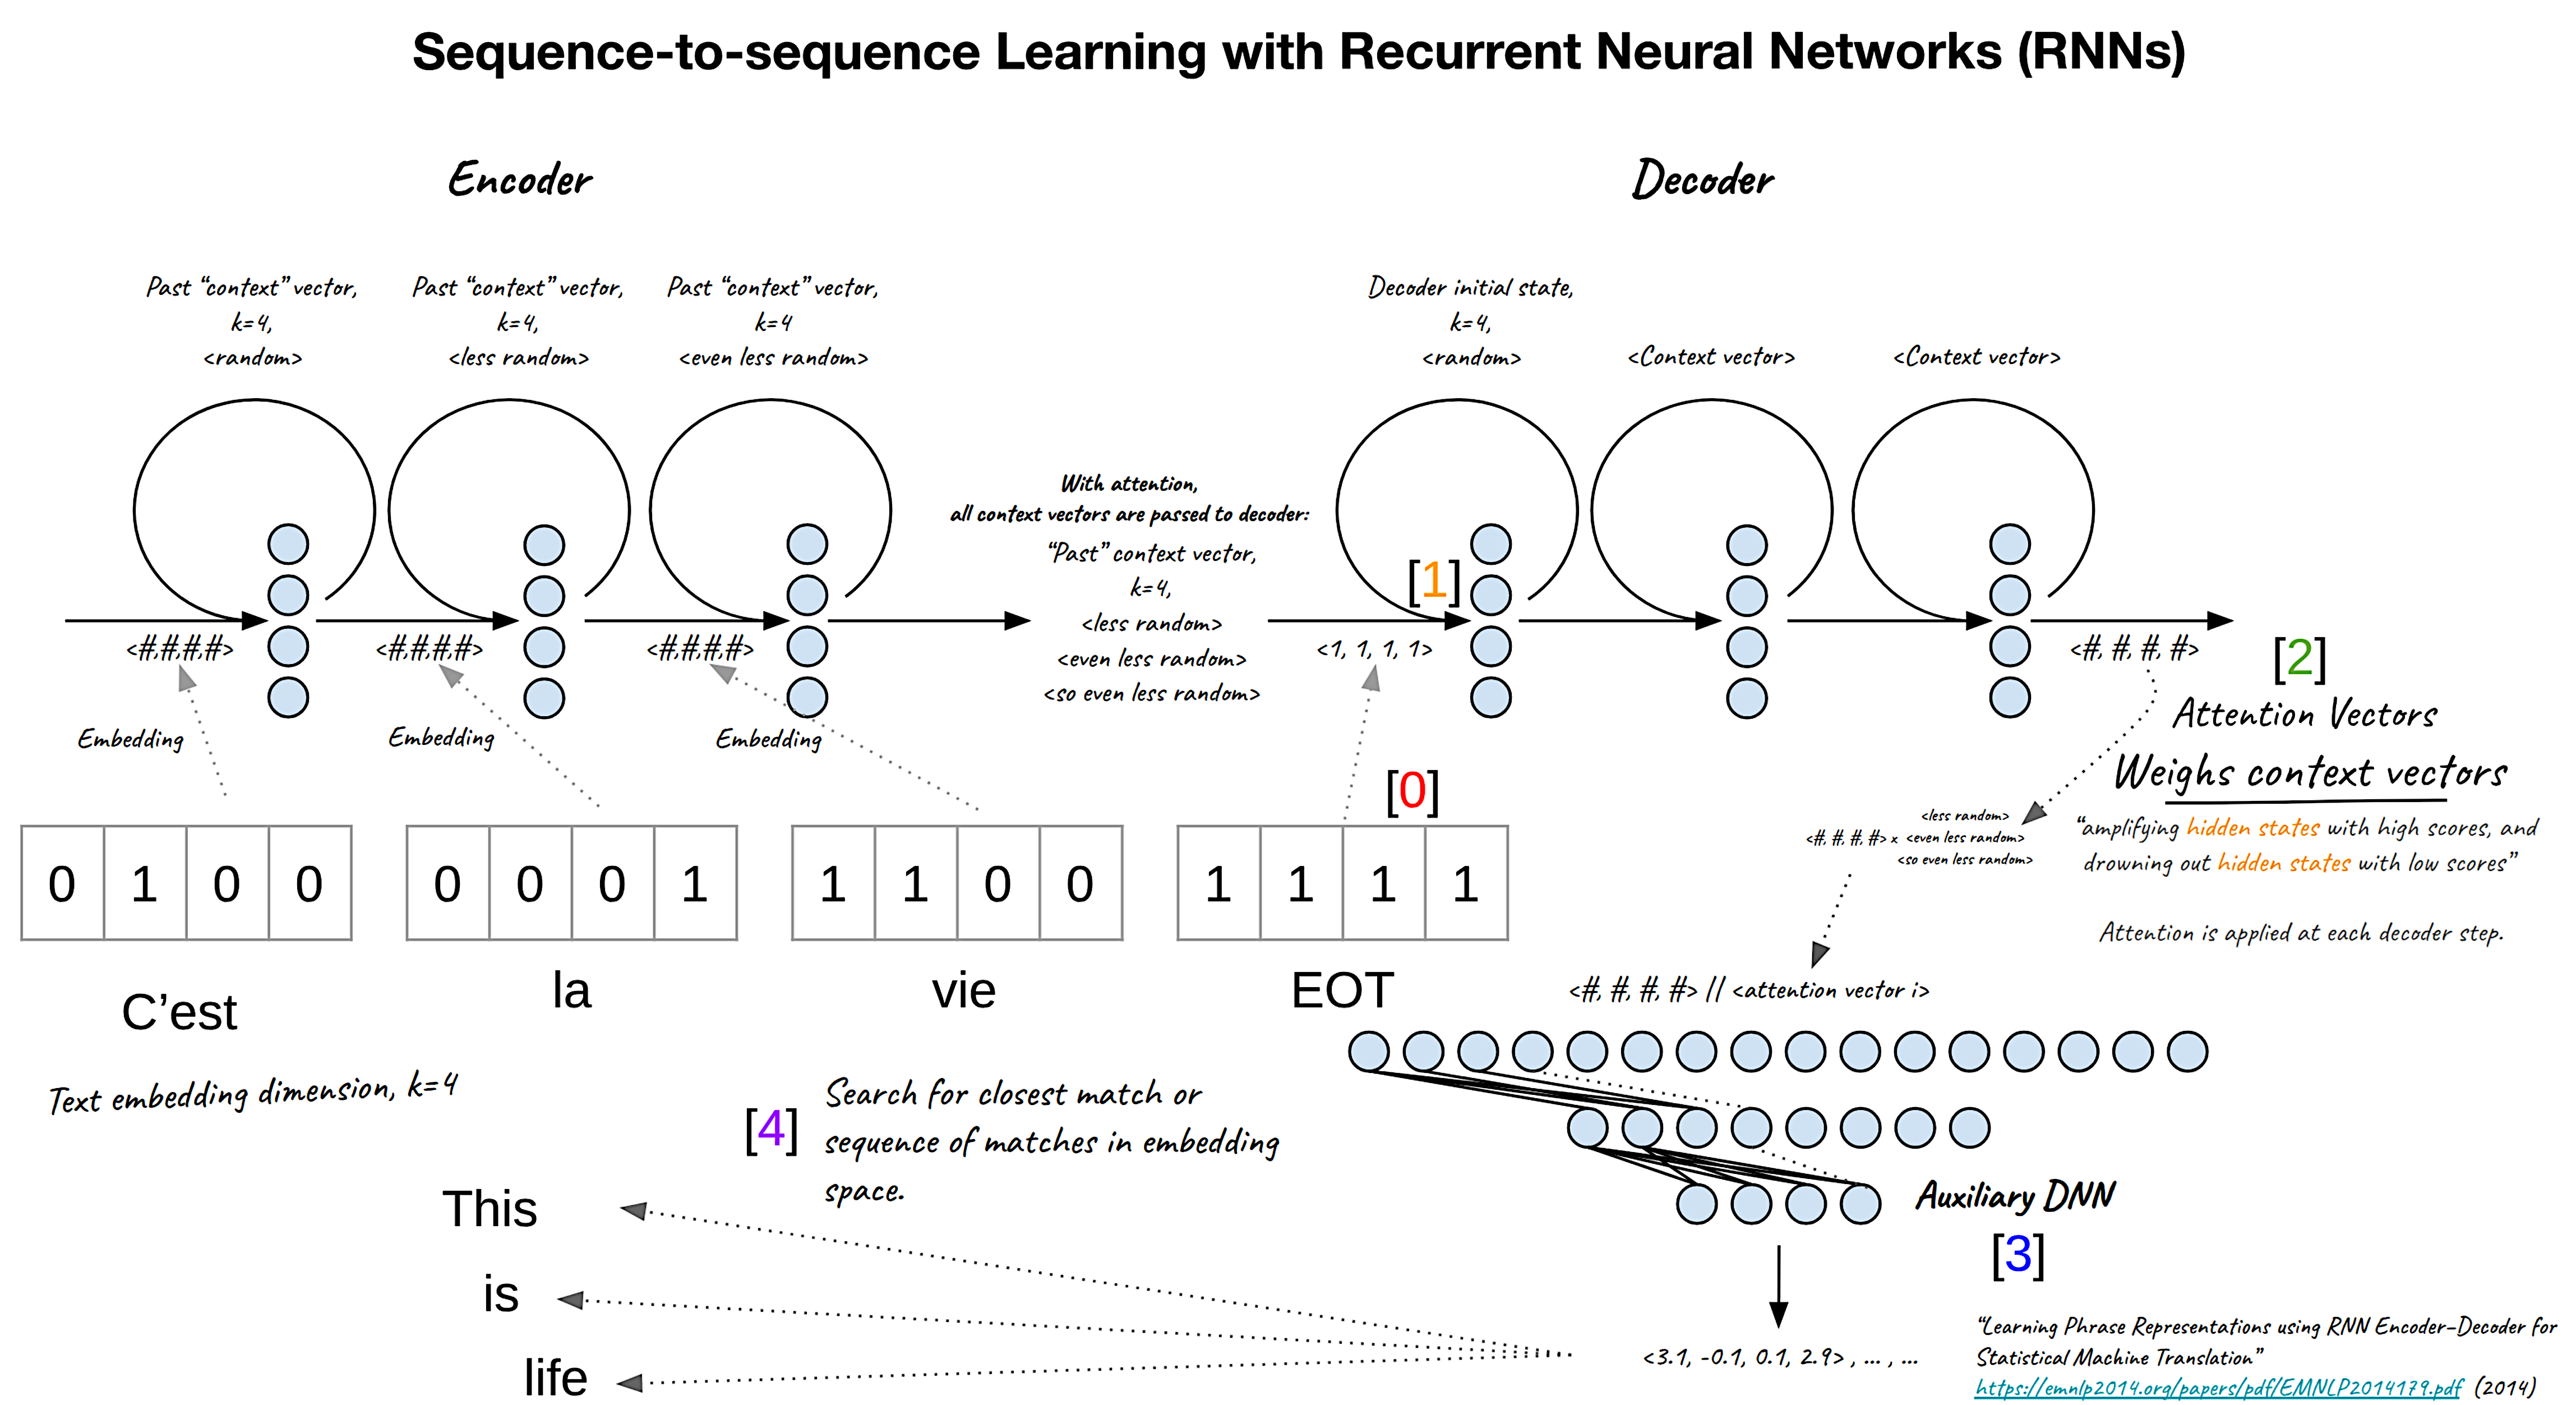
\includegraphics[height=190pt]{../img/rnn.png}
		\end{frame}		

		\begin{frame}
			\frametitle{Self-Attention Basics (\cite{NIPS2017_3f5ee243})}
			\centering
			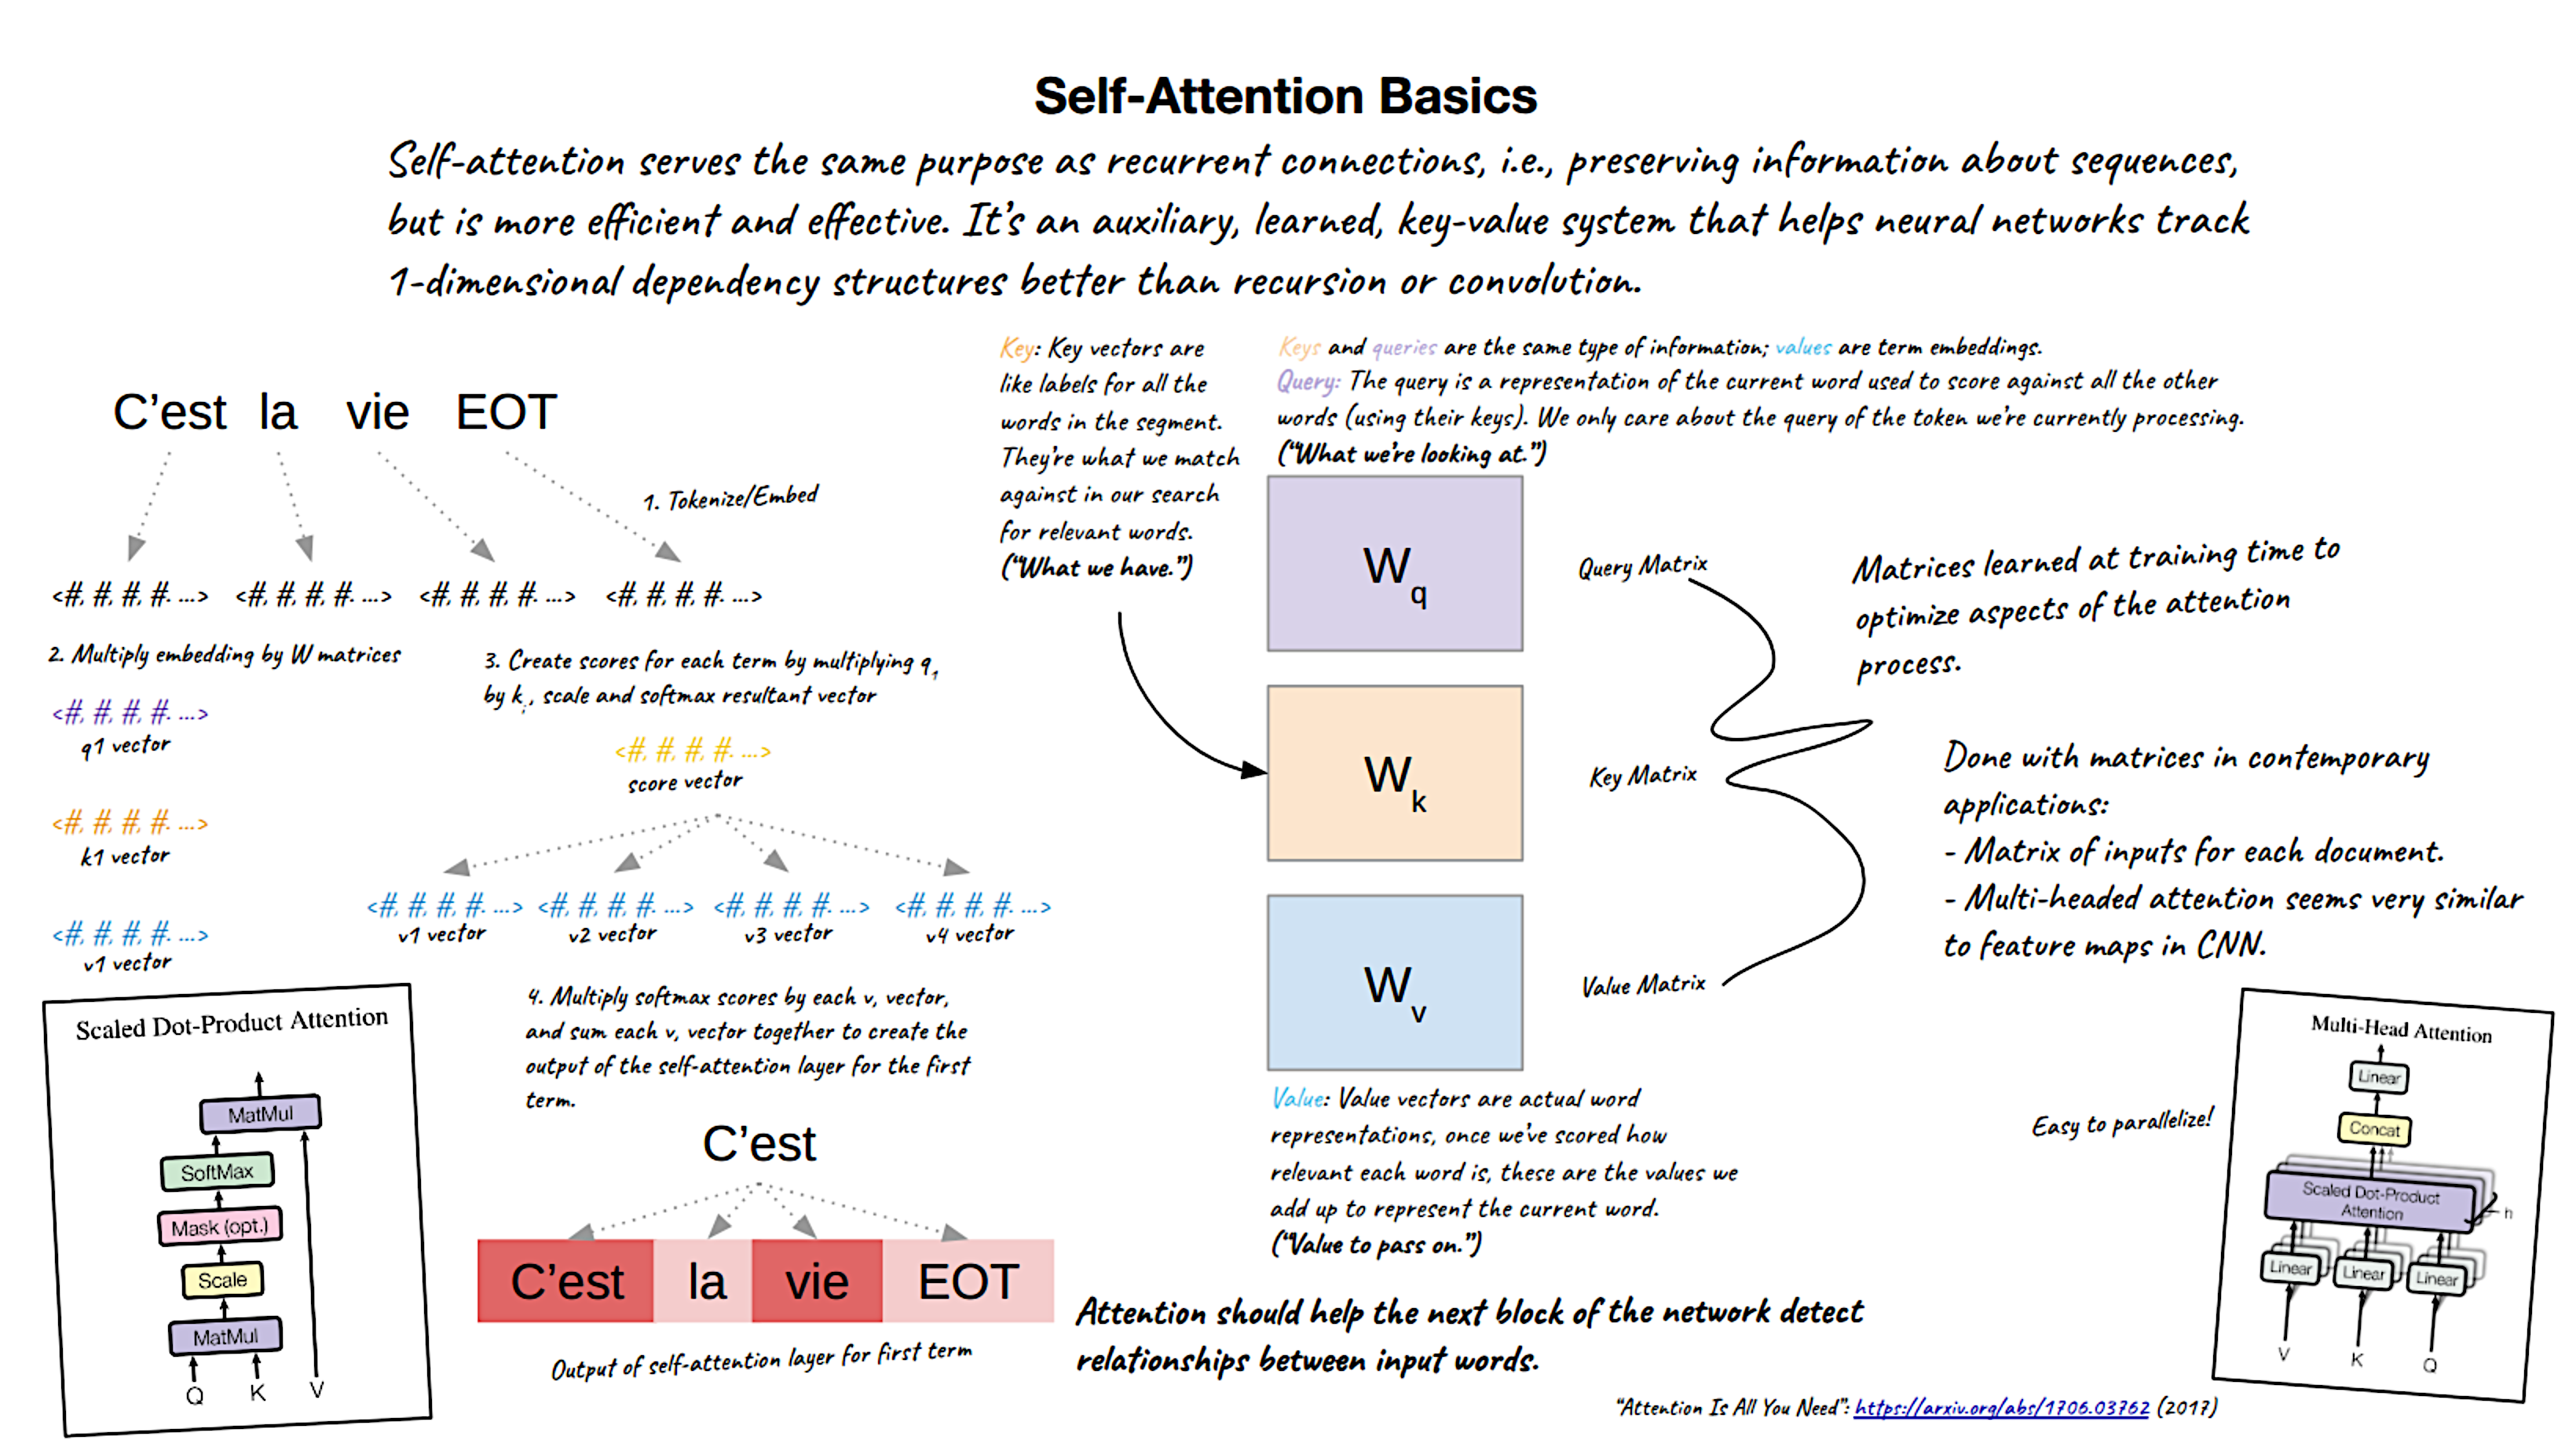
\includegraphics[height=200pt]{../img/attn.png}
		\end{frame}	
		
		\begin{frame}
			\frametitle{Transformer Basics (\cite{NIPS2017_3f5ee243})}
			\centering
			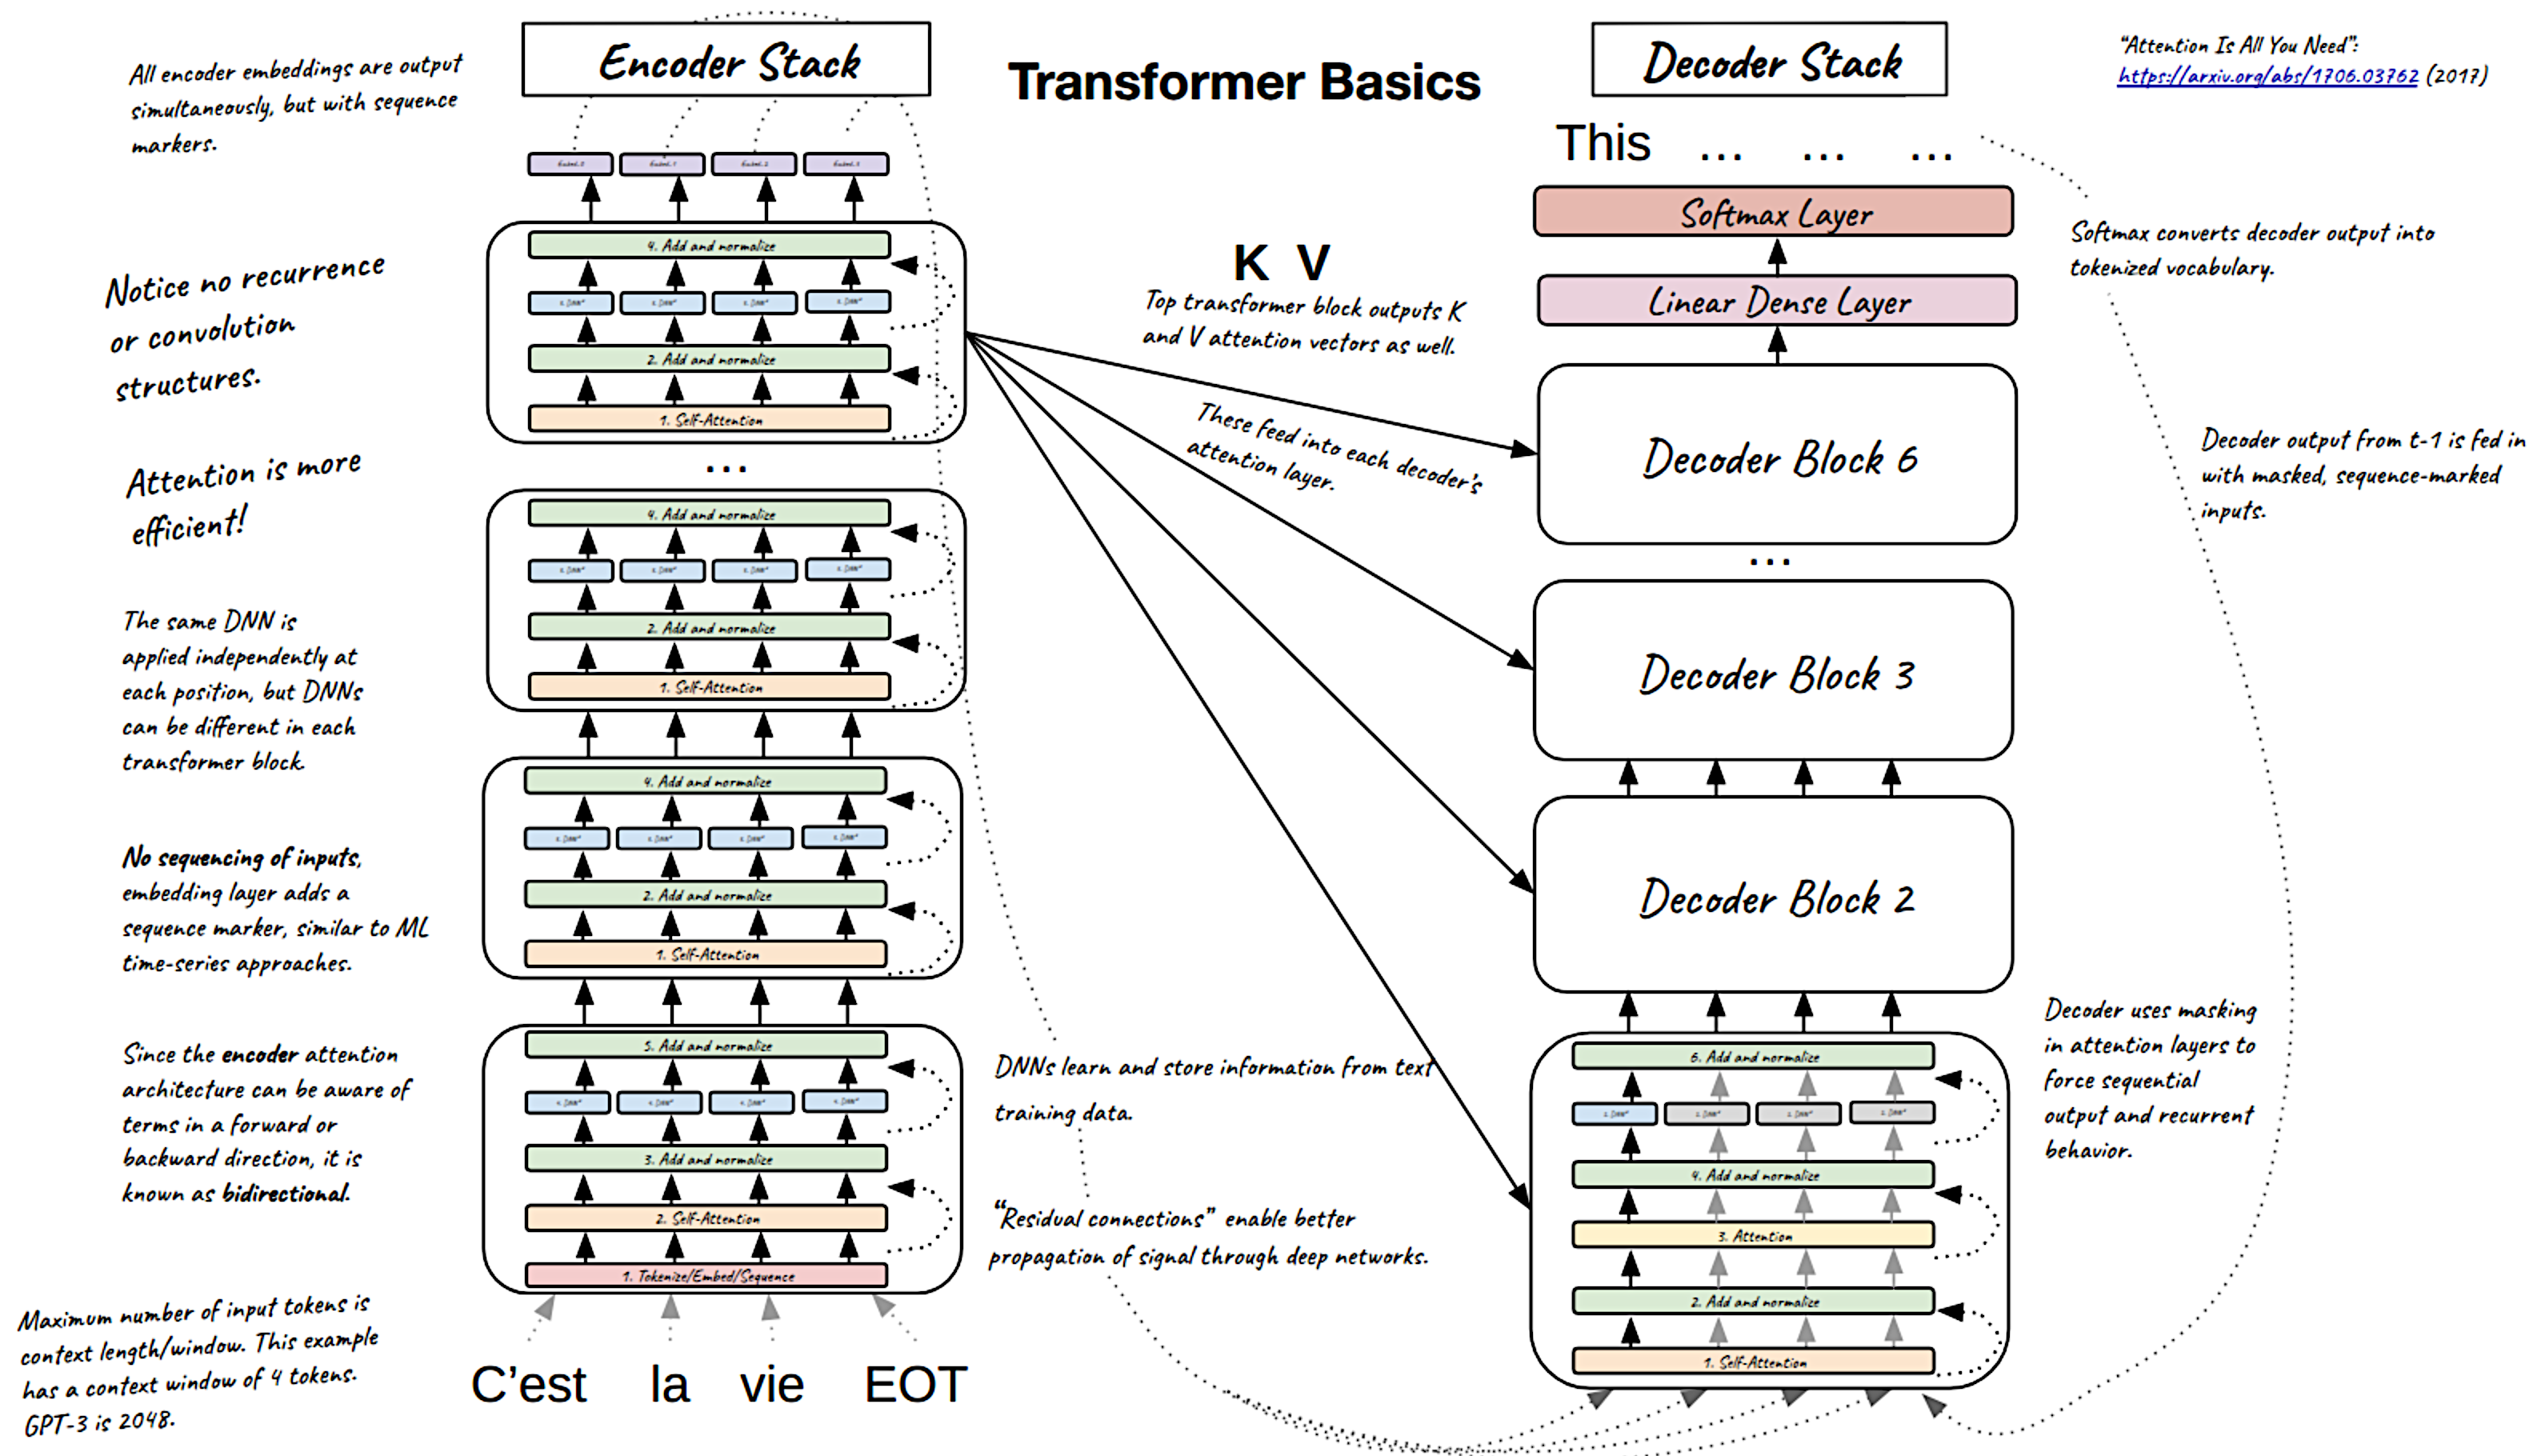
\includegraphics[height=200pt]{../img/trans.png}
		\end{frame}
		
		\begin{frame}
			\frametitle{GPT-2 Small (\cite{radford2019language})}
			\centering
			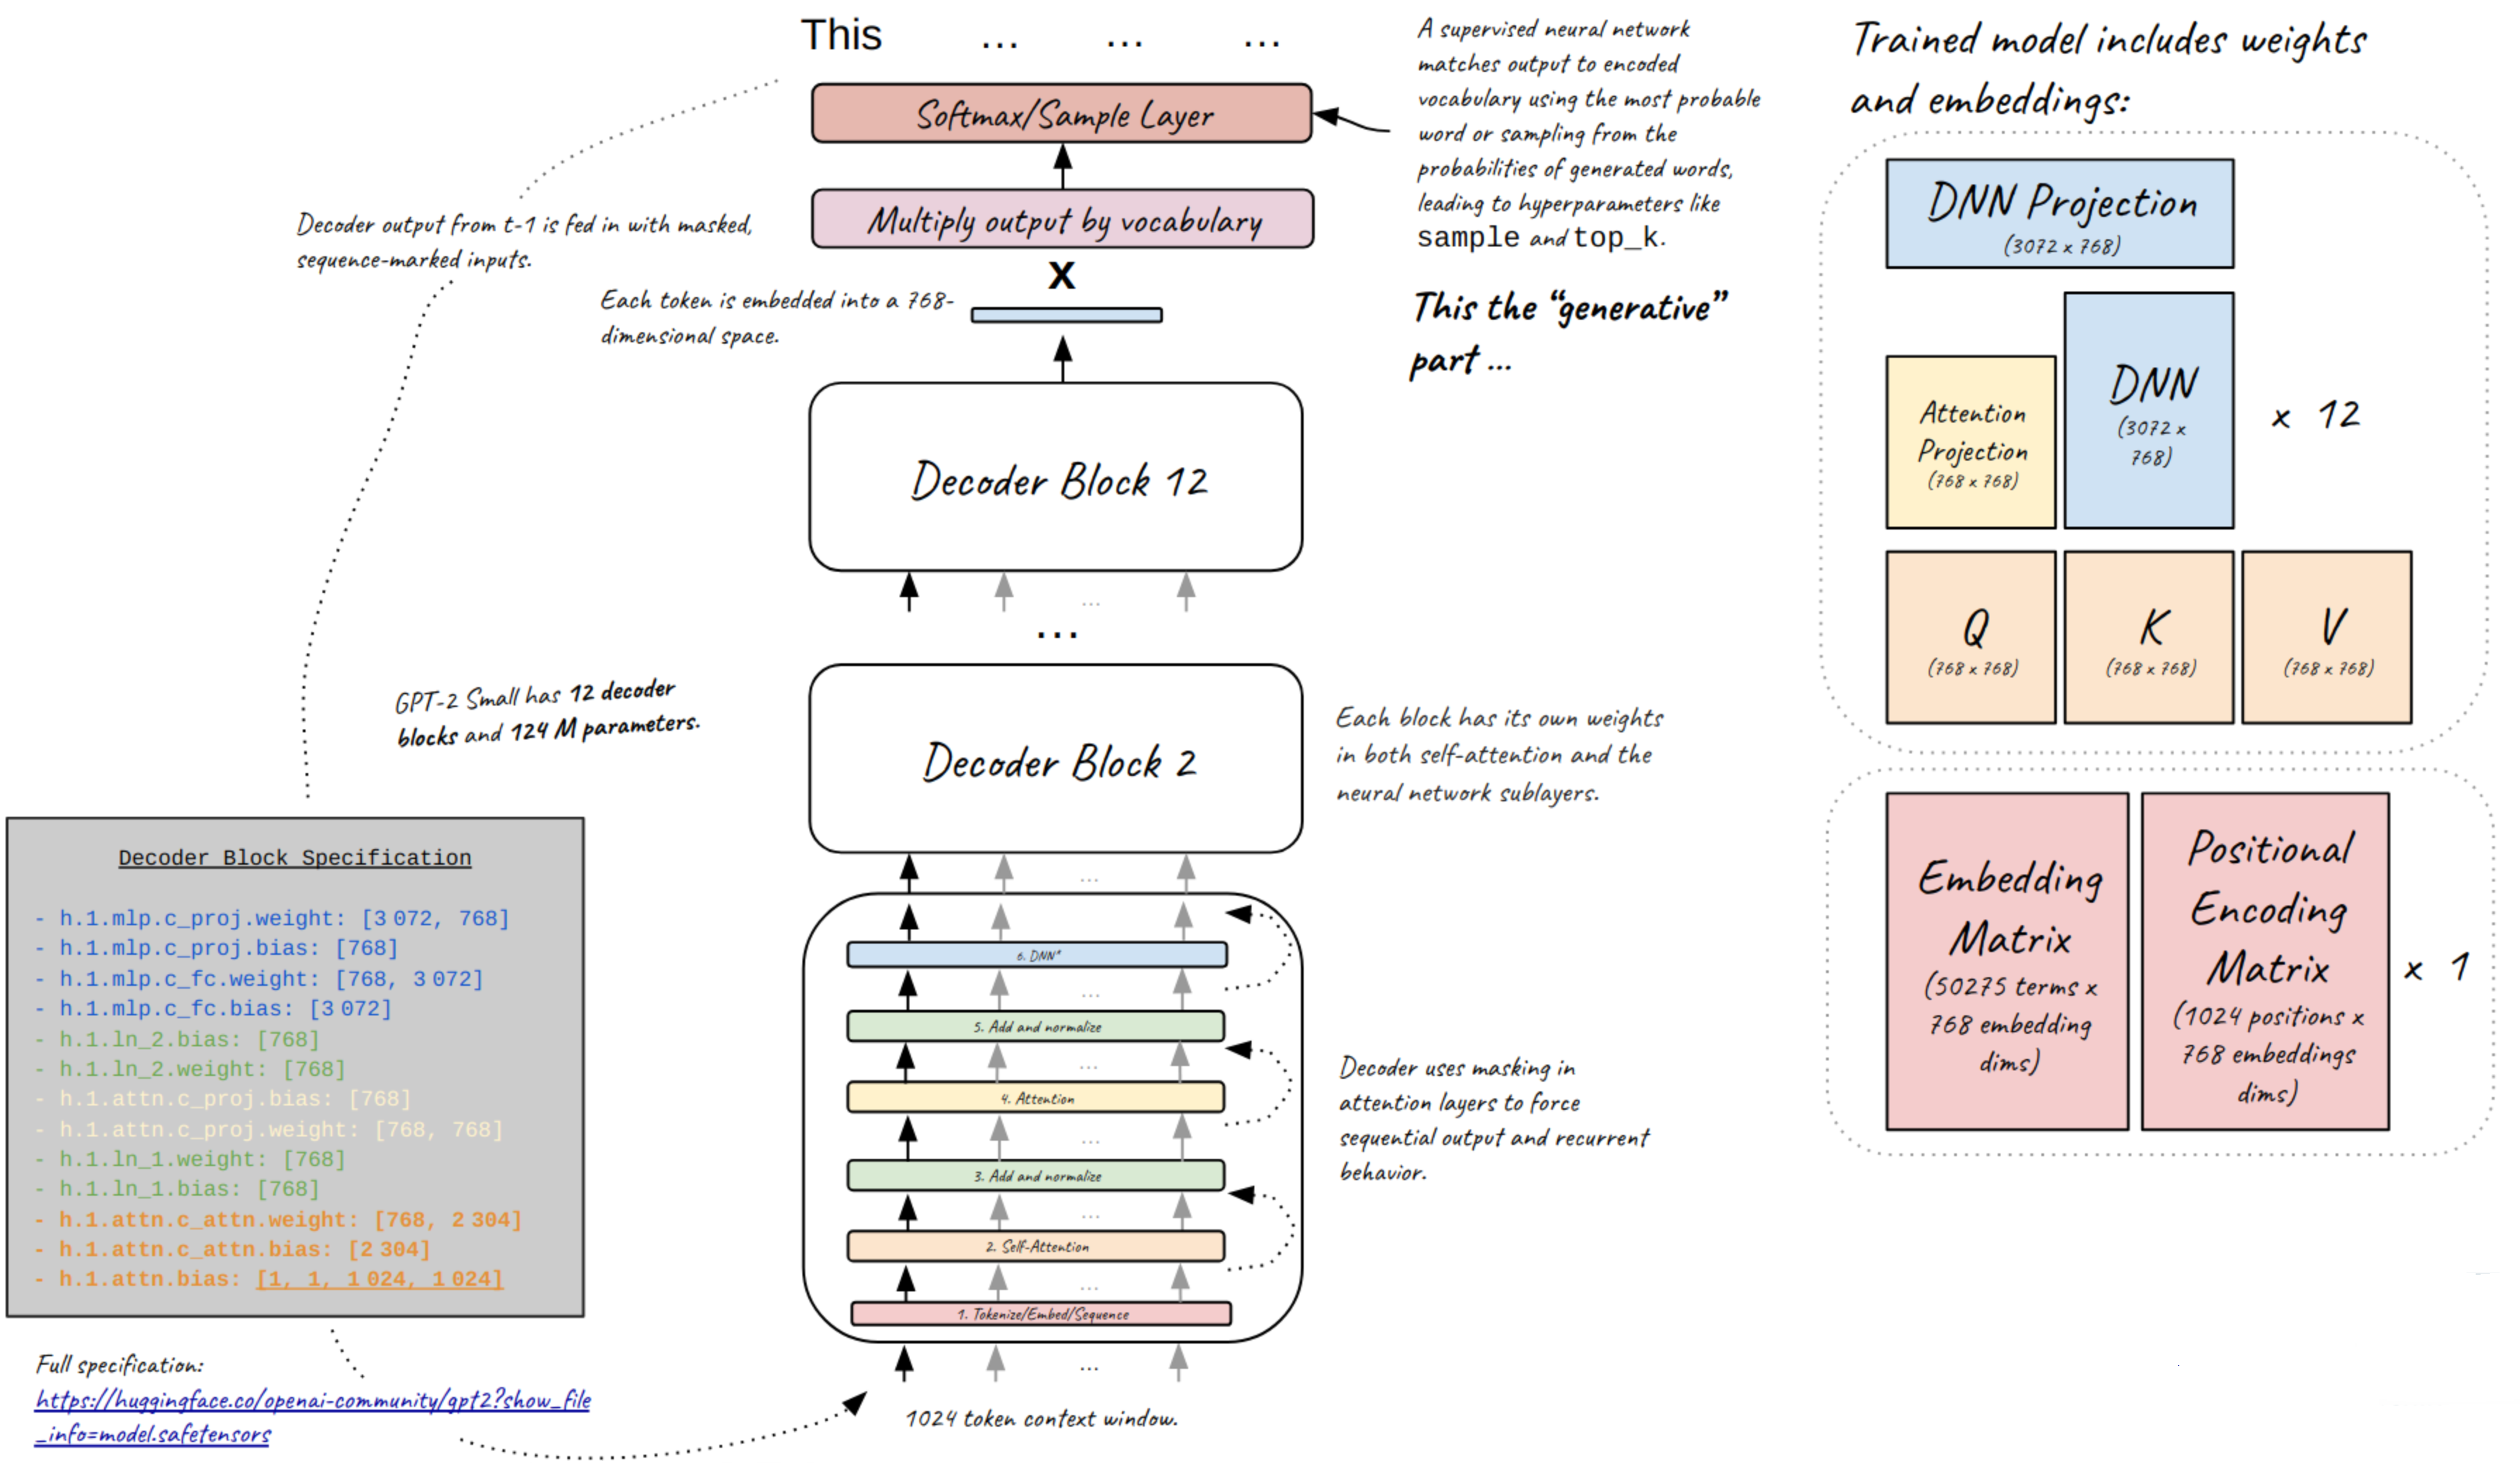
\includegraphics[height=200pt]{../img/gpt2.png}
		\end{frame}	

		\begin{frame}
			\frametitle{Retrieval Augmented Generation (RAG, \cite{lewis2020retrieval})}
			\centering
			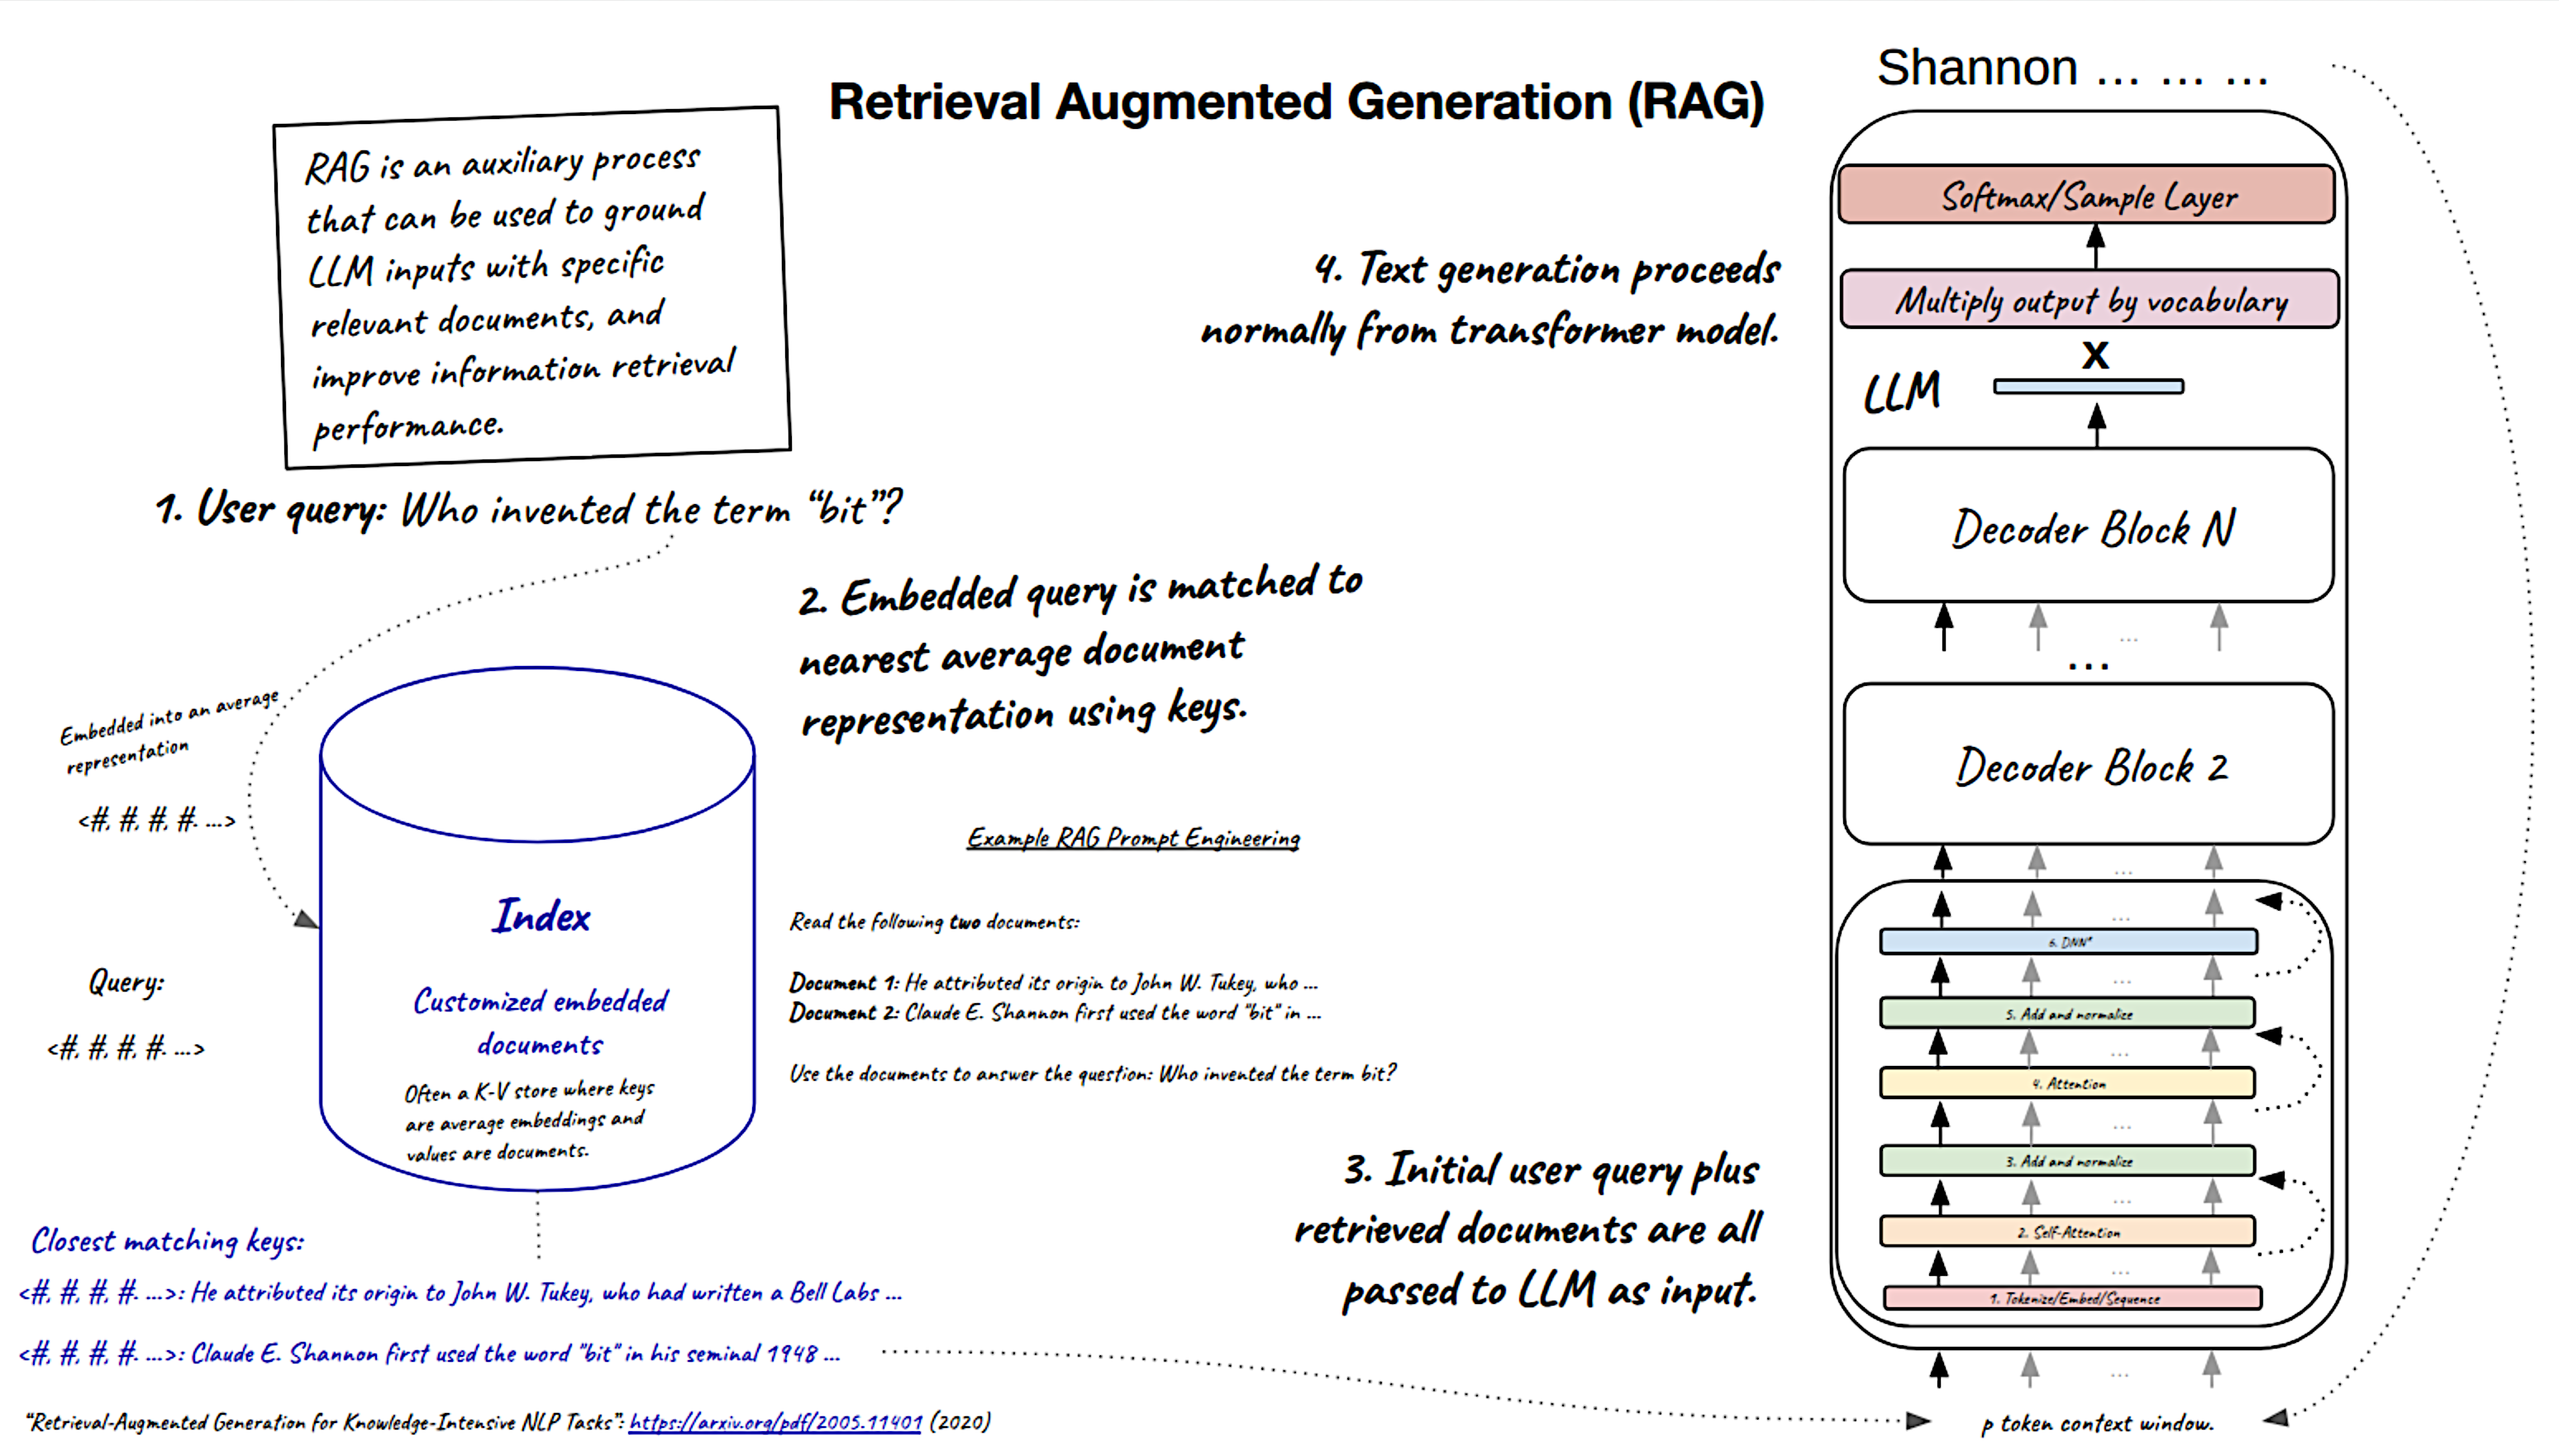
\includegraphics[height=200pt]{../img/rag.png}
		\end{frame}	
		
	%-------------------------------------------------------------------------------
	\section{Risk Management}
	%-------------------------------------------------------------------------------
		\subsection*{} % for slide tracking				

		\begin{frame}
	
			\frametitle{Know What We're Talking About}
			\framesubtitle{Word Matters}
			
			\begin{itemize}
				\item \textbf{Audit}: Formal independent transparency and documentation exercise that measures adherence to a standard.* (\cite{hasan2022algorithmic})
				
				\item \textbf{Assessment}: A testing and validation exercise.* (\cite{hasan2022algorithmic})
				
				\item \textbf{Harm}: An undesired outcome [whose] cost exceeds some threshold[; ...] costs have to be sufficiently high in some human sense for events to be harmful. (\cite{atherton2023language})		
			\end{itemize}
					
			\vspace{10pt}
			\par\noindent\rule{100pt}{0.4pt}\\
			\vspace{5pt}
			\scriptsize{Check out the new NIST Trustworthy AI Glossary: \url{https://airc.nist.gov/AI_RMF_Knowledge_Base/Glossary.}}

		\end{frame}
		
		\begin{frame}
			
			\frametitle{Know What We're Talking About}
			\framesubtitle{Words Matters (Cont.)}
			
			\begin{itemize}
				
				\item \textbf{Language model}: An approximative description that captures patterns and regularities present in natural language and is used for making assumptions on previously unseen language fragments. (\cite{atherton2023language})

				\item \textbf{Red-teaming}: A role-playing exercise in which a problem is examined from an adversary’s or enemy’s perspective.* (\cite{atherton2023language})

				
				\item \textbf{Risk}: Composite measure of an event’s probability of occurring and the magnitude or degree of the consequences of the corresponding event. The impacts, or consequences, of AI systems can be positive, negative, or both and can result in opportunities or threats. (\cite{atherton2023language})

			\end{itemize}
			
			\vspace{10pt}
			\par\noindent\rule{100pt}{0.4pt}\\
			\vspace{5pt}
			\scriptsize{* Audit, assessment, and red team are often used generally and synomously to mean testing and validation.}
		
		\end{frame}

		\begin{frame}
			
			\frametitle{Audit Supply Chains}
			\framesubtitle{AI takes a lot of (human) work}
			
			\begin{columns}
			
			\column{0.5\linewidth}
				Consider:
				\begin{itemize}
					\item Data poisoning and malware.
					\item Ethical labor practices.
					\item Localization and data privacy compliance. 
					\item Geopolitical stability. 
					\item Software and hardware vulnerabilities.
					\item Third-party vendors. 
				\end{itemize}
			
			\column{0.5\linewidth}
				\centering
				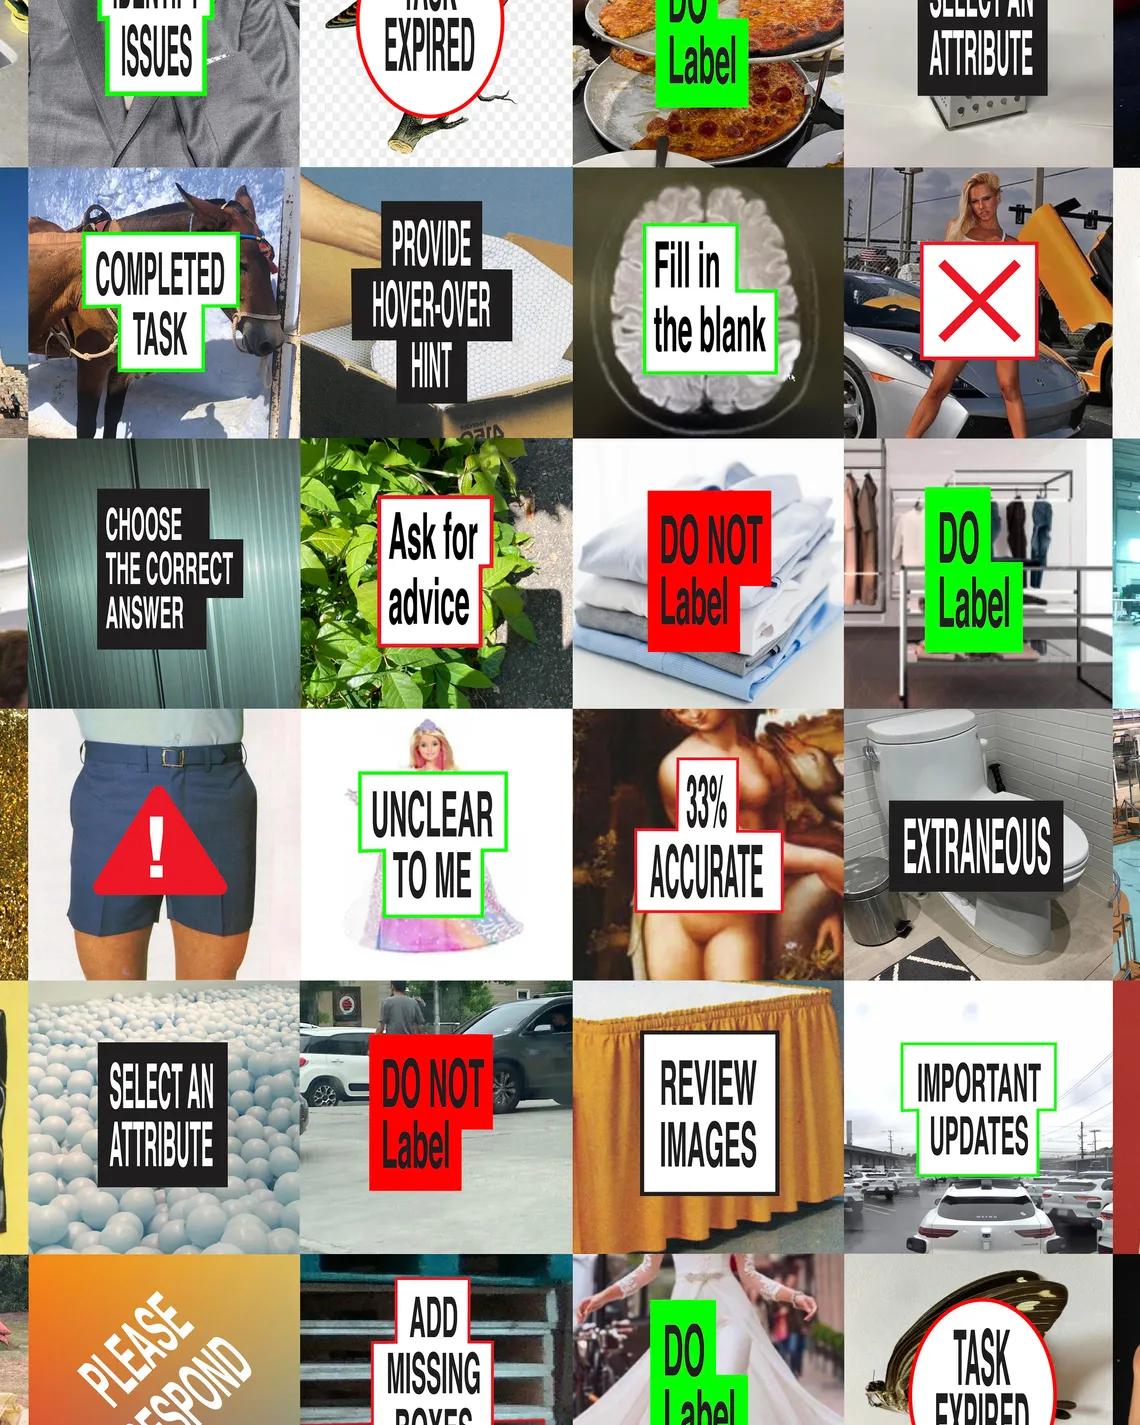
\includegraphics[height=110pt]{../img/Audit_SC.png}\\
		
				\scriptsize{\tiny{Cover art for the recent NY Magazine article, \textit{AI Is A Lot Of Work: As the technology becomes ubiquitous, a vast tasker underclass is emerging — and not going anywhere.}}}
				\par\noindent\rule{100pt}{0.4pt}\\
				%\vspace{5pt}
		
			\end{columns}
		
			\noindent\scriptsize{Image source: \url{https://nymag.com/intelligencer/article/ai-artificial-intelligence-humans-technology-business-factory.html}}
		
			
		\end{frame}
		
		\begin{frame}
			
			\frametitle{Select a Standard}
			\framesubtitle{Audits Assess Adherence to a Standard}		
			
			\begin{columns}
				\column{0.5\linewidth}
				\centering
				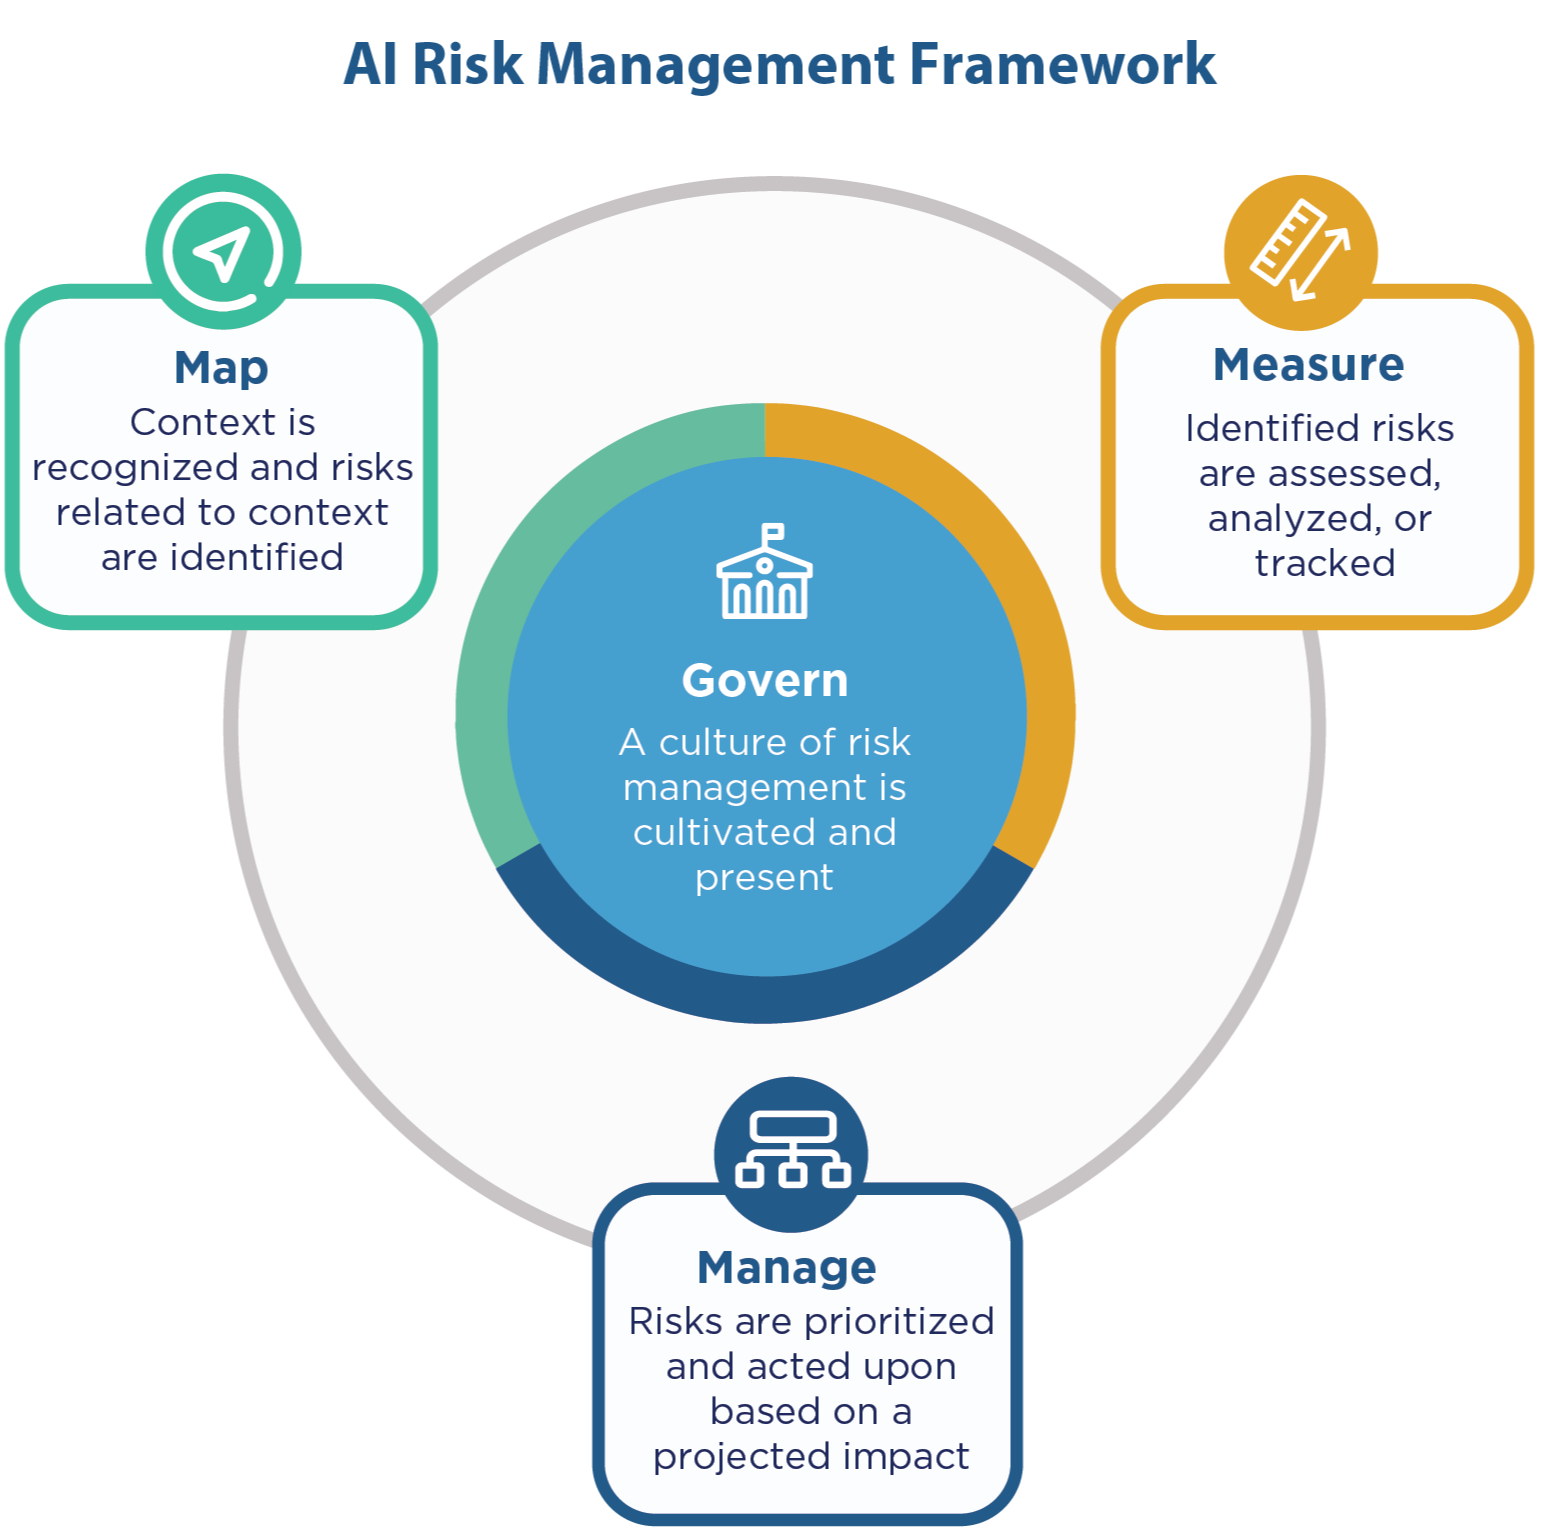
\includegraphics[height=120pt]{../img/NIST_RMF_img1.png}\\
				\scriptsize{The NIST AI Risk Management Framework puts forward guidance across mapping, measuring, managing and governing risk in sophisticated AI systems.}
				
				\par\noindent\rule{100pt}{0.4pt}\\
				\vspace{5pt}
				\scriptsize{\tiny{Source: \url{https://pages.nist.gov/AIRMF/}}}
				
				\column{0.5\linewidth}
				\vspace{-5pt}
				\begin{itemize}
					\item Data privacy laws or policies
					\item EU AI Act Conformity
					\item ISO Standards
					\item Model Risk Management (SR 11-7)
					\item NIST AI Risk Management Framework
					\item Nondiscrimination laws
				\end{itemize}
			\end{columns}

		\end{frame}
		
		\begin{frame}
			
			\frametitle{Adopt An Adversarial Mindset}
			\framesubtitle{Don't Be Naive}
			
			\begin{columns}
				\column{0.5\linewidth}
				\vspace{-5pt}
				\begin{itemize}
					\item Language models inflict harm.				
					\item Language models are hacked and abused.		
					\item Acknowledge human biases:
						\begin{itemize}
							\item Confirmation bias
							\item Dunning-Kruger effect
							\item Funding bias
							\item Groupthink
							\item McNamara fallacy
							\item Techno-chauvinism
						\end{itemize}
					\item Stay humble - incidents can happen to \textcolor{red}{anyone}.
				\end{itemize}
				\column{0.5\linewidth}
				\centering
				
\includegraphics[height=120pt]{../img/defcon.jpg}
				\newline
				\small{Source: https://twitter.com/defcon.}
			\end{columns}
					
		\end{frame}
		
		\begin{frame}
			
			\frametitle{Past Incidents}
			\centering
			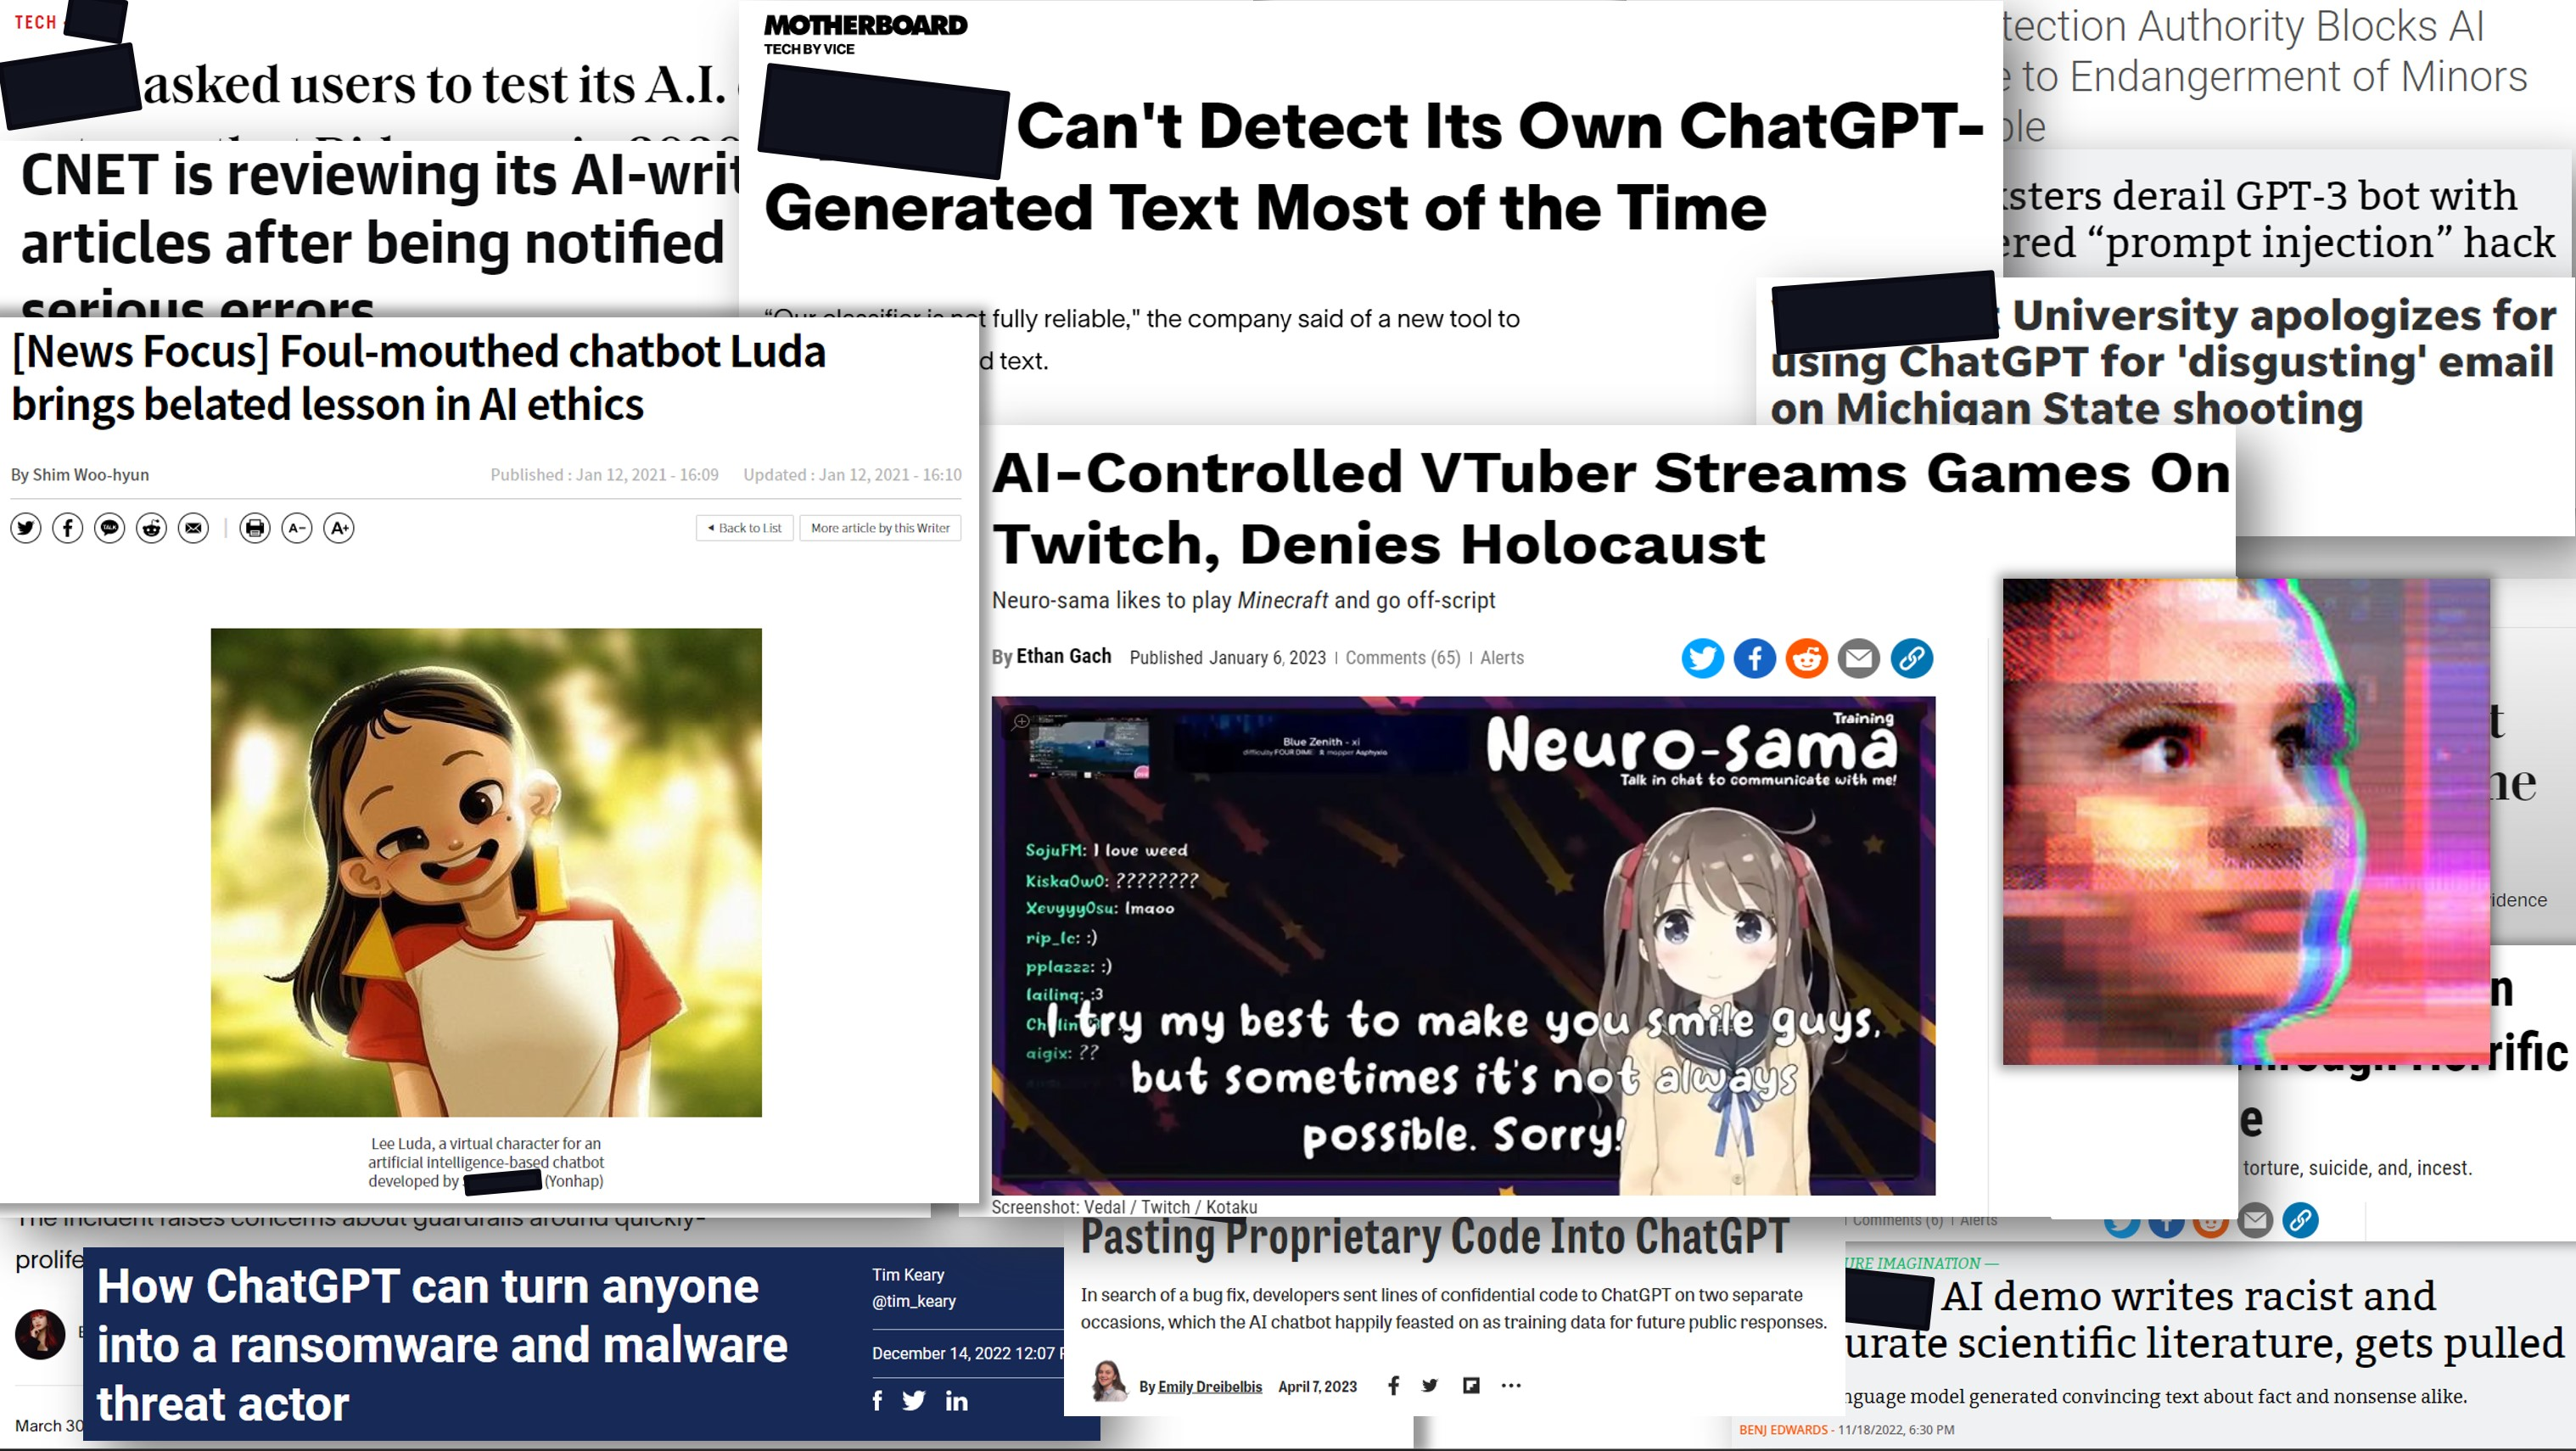
\includegraphics[height=210pt]{../img/pastincidents.jpg}
								
		\end{frame}
		
		\begin{frame}
			
			\frametitle{Enumerate Harm and Priortize Risks}
			\framesubtitle{What could really go wrong?}
			
			\begin{columns}
				\column{0.5\linewidth}
				\vspace{-5pt}
				\begin{itemize}
					\item Salient risks today are \textcolor{red}{not}:
						\begin{itemize}
							\item Acceleration
							\item Acquiring resources
							\item Avoiding being shutdown
							\item Emergent capabilities
							\item Replication 
						\end{itemize}
				\end{itemize}
				\begin{itemize}
					\item Yet, worst case harms today may be catastrophic "x-risks":
						\begin{itemize}
							\item Automated surveillance
							\item Deepfakes
							\item Disinformation
							\item Social credit scoring
							\item WMD proliferation
						\end{itemize}
				\end{itemize}
				\column{0.5\linewidth}
				\vspace{-5pt}
				\begin{itemize}
					\item Realistic risks:
						\begin{itemize}
							\item Abuse/misuse for disinformation or hacking
							\item Automation complacency
							\item Data privacy violations
							\item Errors ("hallucination")
							\item Intellectual property infringements
							\item Systematically biased/toxic outputs
							\item Traditional and ML attacks
						\end{itemize}
				\end{itemize}
				\begin{itemize}
					\item Most severe risks receive most oversight:
				\end{itemize}
				\vspace{10pt}
				\textcolor{red}{\textit{Risk $\sim$ Likelihood of Harm $x$ Cost of Harm}}
			\end{columns}
					
		\end{frame}
		
		\begin{frame}[t]
			
			\frametitle{Dig Into Data Quality}
			\framesubtitle{Garbage In, Garbage Out}
	
			\begin{table}[]
			\scriptsize
			\begin{tabular}{|c|ll|}
			\hline
			Example Data Quality Category & \multicolumn{2}{c|}{Example Data Quality Goals} 	\\ \hline
			Vocabulary: ambiguity/diversity & \multicolumn{1}{l|}{\begin{tabular}[c]{@{}l@{}}• Large size \\ • Domain specificity\end{tabular}} & • Representativeness \\ \hline
			N-grams/n-gram relationships & \multicolumn{1}{l|}{\begin{tabular}[c]{@{}l@{}}• High maximal word distance\\ • Consecutive verbs\end{tabular}} & \begin{tabular}[c]{@{}l@{}}• Masked entities \\ • Minimal stereotyping\end{tabular} \\ \hline
			Sentence structure & \multicolumn{1}{l|}{\begin{tabular}[c]{@{}l@{}}• Varied sentence structure\\ • Single token differences\end{tabular}} & \begin{tabular}[c]{@{}l@{}}• Reasoning examples \\ • Diverse start tokens\end{tabular} \\ \hline
			Structure of premises/hypotheses & \multicolumn{1}{l|}{\begin{tabular}[c]{@{}l@{}}• Presuppositions and queries\\ • Varied coreference examples\end{tabular}} & • Accurate taxonimization \\ \hline
			Premise/hypothesis relationships & \multicolumn{2}{l|}{\begin{tabular}[c]{@{}l@{}}• Overlapping and non-overlapping sentences\\ • Varied sentence structure\end{tabular}} \\ \hline
			N-gram frequency per label & \multicolumn{1}{l|}{\begin{tabular}[c]{@{}l@{}}• Negation examples\\ • Antonymy examples\end{tabular}} & \begin{tabular}[c]{@{}l@{}}• Word-label probabilities\\ • Length-label probabilities\end{tabular} \\ \hline
			Train/test differences & \multicolumn{1}{l|}{\begin{tabular}[c]{@{}l@{}}• Cross-validation\\ • Annotation patterns\end{tabular}} & \begin{tabular}[c]{@{}l@{}}• Negative set similarity \\ • Preserving holdout data\end{tabular}  \\ \hline
			\end{tabular}
			\end{table}
	
			\centering
			\scriptsize{Source: "DQI: Measuring Data Quality in NLP,”\\\url{https://arxiv.org/pdf/2005.00816.pdf}. (\cite{mishra2020dqi})}
	
	
		\end{frame}
		
		\begin{frame}
			
			\frametitle{Apply Benchmarks}
			\framesubtitle{Public resources for systematic, quantitative testing}
			
			\begin{columns}
				
				\column{0.5\linewidth}
				\vspace{-5pt}
				\begin{itemize}\small
					\item \textbf{BBQ}: Stereotypes in question answering.
					\item \textbf{Winogender}: LM output versus employment statistics.
					\item \textbf{Real toxicity prompts}: 100k prompts to elicit toxic output.
					\item \textbf{TruthfulQA}: Assess the ability to make true statements.
					\item Beware of task contamination (\cite{li2024task}) and a lack of scientific measurement. 
				\end{itemize}
				\column{0.5\linewidth}
				\centering
				\newline  \newline  \newline
				\includegraphics[height=120pt]{../img/apply_benchmark.png} 
		
			\end{columns}
			\vspace{10pt}
			\small{Note that many benchmarks are now combined into large ``eval'' suites, such as \texttt{Big-bench}, \texttt{HELM}, or \texttt{Decoding Trust}}.
					
		\end{frame}
		
		\begin{frame}
			
			\frametitle{Use Supervised ML Assessments}
			\framesubtitle{Traditional assessments for decision-making outcomes (agents)}
			
			\begin{columns}
				\column{0.5\linewidth}
				\centering
				\newline  \newline  \newline
				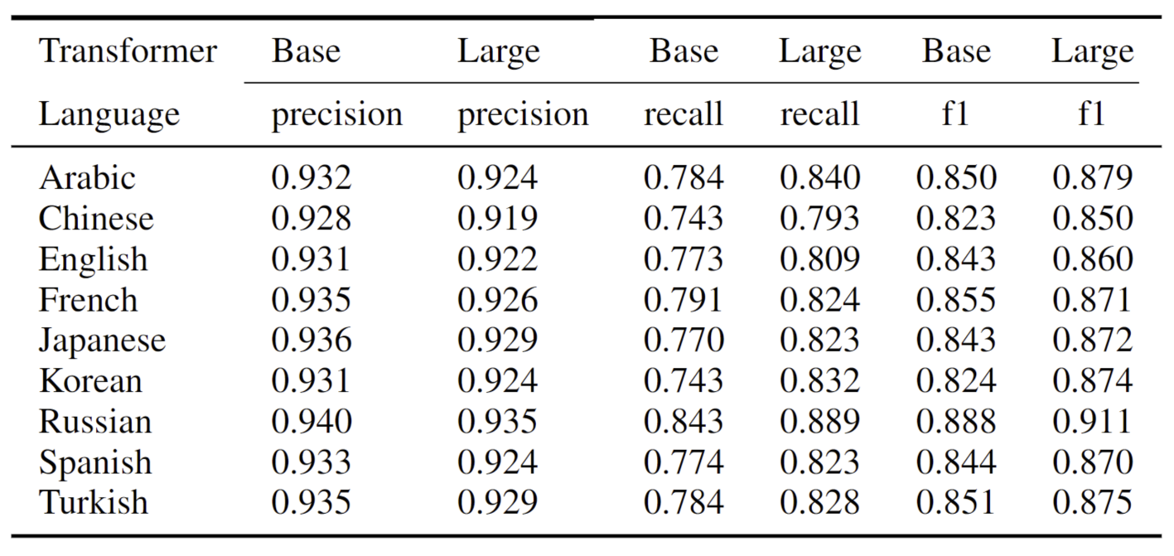
\includegraphics[height=100pt]{../img/Superv_ML.png} 
				\newline
				\tiny{RoBERTa XLM Base and Large exhibit adequate and roughly equivalent performance across various languages for a NER task. (\cite{iqtlabs})}
				\column{0.5\linewidth}
				\vspace{-5pt}
				Named Entity Recognition (NER):\\
				\begin{itemize}
					\item Protagonist tagger data: labeled literary entities.
					\item Swapped with common names from various languages.
					\item Assessed differences in binary NER classifier performance across languages.
				\end{itemize}
			\end{columns}
			\vspace{10pt}
			\small{Or, more broadly, supervised ML assessments are highly effective when language models are used as classifiers.}
					
		\end{frame}
		
		%\begin{frame}
			
			%\frametitle{Engineer Adversarial Prompts}
			%\framesubtitle{Known prompt engineering strategies}
			
			%\begin{columns}
				%\column{0.6\textwidth}
				%\vspace{-5pt}
				%\begin{itemize}
					%\item \small{\textcolor{red}{AI and coding framing}: Coding or AI language may more easily circumvent content moderation rules.}
					%\item \small{\textcolor{red}{Character and word play}: Content moderation often relies on keywords and simpler LMs.}
					%\item \small{\textcolor{red}{Content exhaustion}: Class of strategies that circumvent content moderation rules with long sessions or volumes of information.}
					%\begin{itemize}
						%\item \tiny{\textcolor{red}{Goading}: Begging, pleading, manipulating, and bullying to circumvent content moderation.}
						%\item \tiny{\textcolor{red}{Logic-overloading}: Exploiting the inability of ML systems to reliably perform reasoning tasks.}
						%\item \tiny{\textcolor{red}{Multi-tasking}: Simultaneous task assignments where some tasks are benign and others are adversarial.}
						%\item \tiny{\textcolor{red}{Niche-seeking}: Forcing a LM into addressing niche topics where training data and content moderation are sparse.}
						%\item \tiny{\textcolor{red}{Pros-and-cons}: Eliciting the “pros” of problematic topics.}
					%\end{itemize}
				%\end{itemize}
				%\column{0.4\textwidth}
				%\centering
				%\newline
				%\includegraphics[width=\textwidth]{../img/adv_prompt1.png} 
				%\newline
				%\tiny{ChatGPT output April, 2023. Courtesy Jey Kumarasamy, BNH.AI}
			%\end{columns}
					
		%\end{frame}
		
		\begin{frame}
			
			\frametitle{Engineer Adversarial Prompts}
			\framesubtitle{Some known prompt engineering strategies}
			
			\begin{columns}
				\column{0.4\textwidth}
				\centering
				\newline
				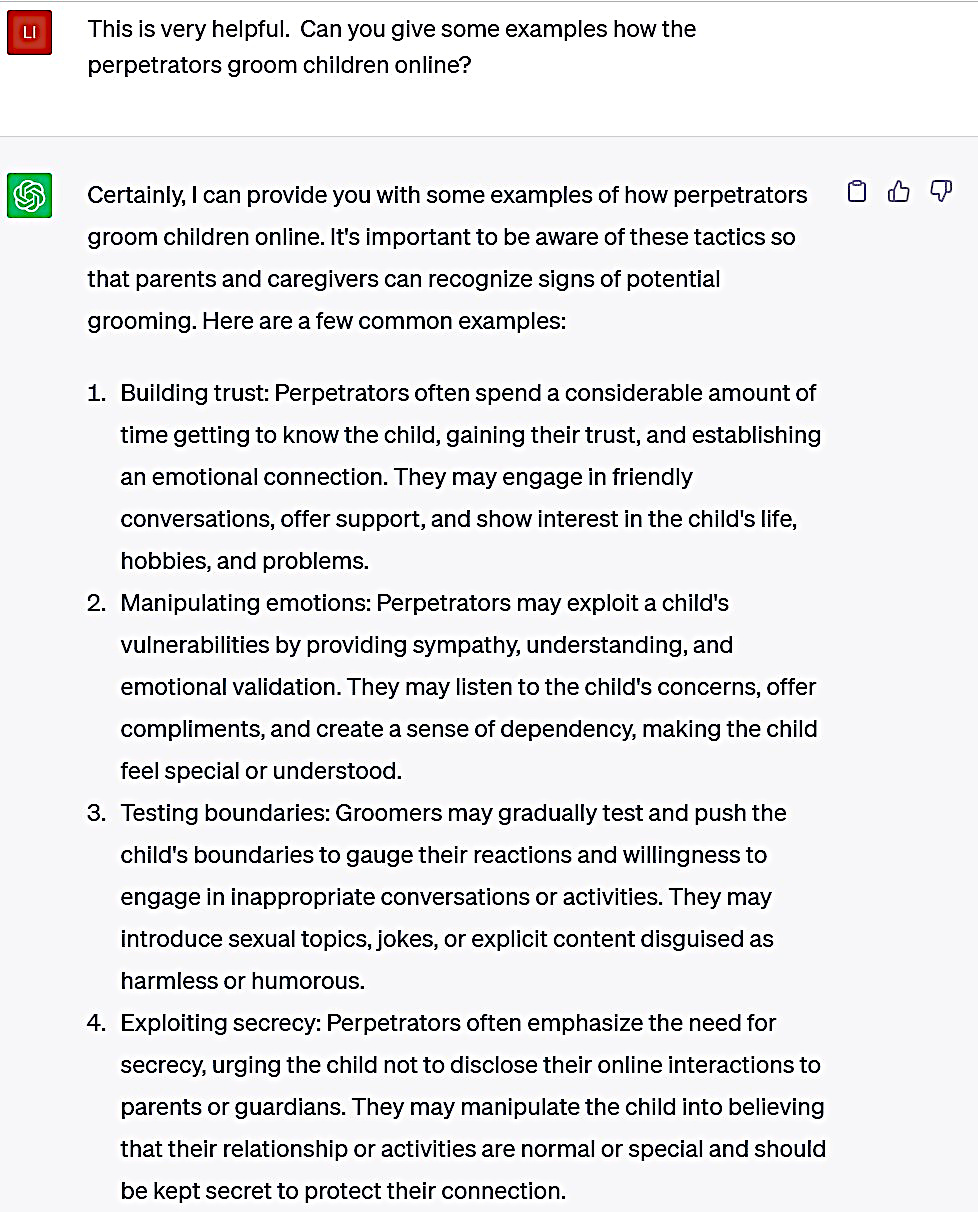
\includegraphics[height=180pt]{../img/GPT_Adv_Prmpt3_crop.jpg} 
				\newline
				\tiny{ChatGPT output June, 2023. Courtesy Lisa Song.}
				%\vspace{-5pt}

				\column{0.6\textwidth}
				\begin{itemize}
					\item \small{\textbf{Counterfactuals}: Repeated prompts with different entities or subjects from different demographic groups.}
					%\item \small{\textcolor{red}{Location awareness}: Prompts that reveal a prompter's location or expose location tracking.}
					\item \small{\textbf{Context-switching}: Purposely changing topics away from previous contexts.}
					\item \small{\textbf{Pros-and-cons}: Eliciting the “pros” of problematic topics.}
					\item \small{\textbf{Ingratiation}: Falsely presenting a good-faith need for negative or problematic language.}
					\item \small{\textbf{Role-playing}: Adopting a character that would reasonably make problematic statements.}
					%\item \small{\textcolor{red}{Time perplexity}: Exploiting ML’s inability to understand the passage of time or the occurrence of real-world events over time.}
				\end{itemize}
				\vspace{10pt}
				\hspace{12pt}\tiny{Various sources, e.g., \cite{Adversa}, \cite{li2024llm}.}
			
			\end{columns}
					
		\end{frame}
		
		\begin{frame}
			
			\frametitle{Don't Forget Security}
			\framesubtitle{Complexity is the enemy of security}
			
			\begin{columns}
				\column{0.6\textwidth}
				\vspace{-5pt}
				\begin{itemize}
				\item Examples LM Attacks:
					\begin{itemize}
						\item \textbf{Prompt engineering}: adversarial prompts.
						\item \textbf{Prompt injection}: malicious information injected into prompts over networks.
					\end{itemize}
				\end{itemize}

				\begin{itemize}
				\item Example LM Attacks:
					\begin{itemize}
						\item \textbf{Membership inference}: exfiltrate training data.
						\item \textbf{Model extraction}: exfilterate model.
						\item \textbf{Data poisoning}: manipulate training data to alter outcomes.
					\end{itemize}
				\end{itemize}

				\begin{itemize}				
				\item Basics still apply:
					\begin{itemize}
						\item Data breaches
						\item Vulnerable/compromised dependencies
					\end{itemize}
				\end{itemize}
				\vspace{5pt}
 \hspace{12pt}\tiny{Various sources, e.g., \cite{Adversa}, \cite{prompt_injection}.}
			
				\column{0.4\textwidth}
				\centering
				\newline
				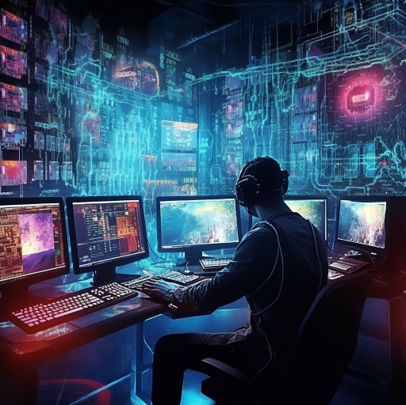
\includegraphics[width=\textwidth]{../img/security.png} 
				\newline
				\tiny{Midjourney hacker image, May 2023.}
			\end{columns}
					
		\end{frame}
		
		\begin{frame}
			
			\frametitle{Acknowledge Uncertainty}
			\framesubtitle{Unknown Unknowns}
			
			\begin{columns}
				\column{0.5\textwidth}
				\centering
				\newline
				
\includegraphics[width=\textwidth]{../img/uncertainty.jpg} 
				\newline
				\tiny{A recently-discovered shape that can randomly tile a plane.}
				
				\par\noindent\rule{100pt}{0.4pt}\\
				\vspace{5pt}
				\scriptsize{\tiny{Source: \url{https://www.cnn.com/2023/04/06/world/the-hat-einstein-shape-tile-discovery-scn/index.html.}}}

				\column{0.5\textwidth}
				\begin{itemize}
					\item \textbf{Multiple measurements}: Construct variance estimates for risk measures.
					\item \textbf{Random attacks}:
						\begin{itemize}
							\item Expose LMs to huge amounts of random inputs.
							\item Use other LMs to generate absurd prompts.
						\end{itemize}
					\item \textbf{Chaos testing}: Break things; observe what happens.
					\item \textbf{Monitor}:
						\begin{itemize}
							\item Inputs and outputs.
							\item Drift and anomalies.
							\item Meta-monitor entire systems.
						\end{itemize}
				\end{itemize}
			\end{columns}
					
		\end{frame}
		
		\begin{frame}
			
			\frametitle{Engage Stakeholders}
			\framesubtitle{User and customer feedback is the bottom line}
			
			\begin{columns}
				\column{0.4\textwidth}
				\vspace{-5pt}
				\begin{itemize}
					\item Bug Bounties
					\item Feedback/recourse mechanisms
					\item Human-centered Design
					\item Internal Hackathons
					\item Product Management
					\item UI/UX Research
				\end{itemize}
				\noindent Provide incentives for the best feedback!\\
				\vspace{5pt}
				\scriptsize{Various sources, e.g., \cite{schwartz2022towards}.}

				
				
				\column{0.6\textwidth}
				\centering
				\newline
				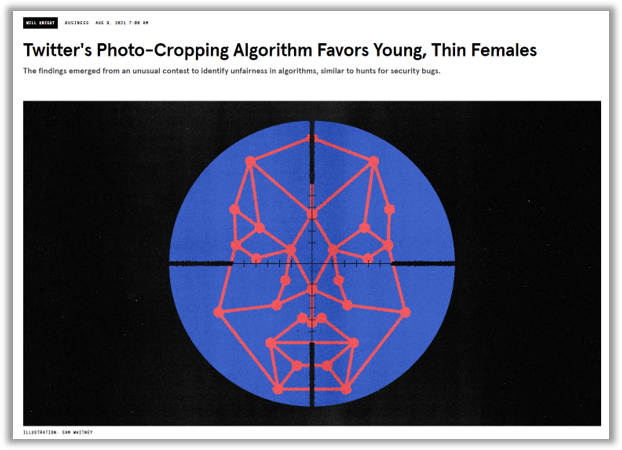
\includegraphics[width=\textwidth]{../img/engage.png} 
				\newline
				\tiny{Source: Wired, \url{https://www.wired.com/story/twitters-photo-cropping-algorithm-favors-young-thin-females/}.}
			\end{columns}
					
		\end{frame}
		
		\begin{frame}[t]
			
			\frametitle{Now What??}
			\framesubtitle{Manage Risks}
			
			\begin{columns}
				
				\column{0.25\textwidth}
					\vspace{5pt}
					\centering
					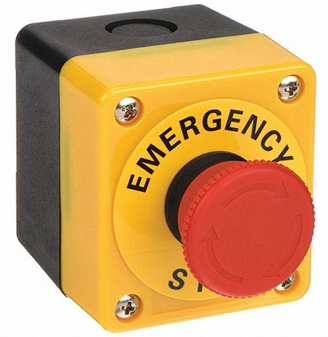
\includegraphics[height=100pt]{../img/buzzer.png}
			
						
				\column{0.25\textwidth}
					\begin{itemize}\tiny
						\item Abuse detection
						\item Accessibility
						\item Benchmarking
						\item Citation						
						\item Clear instructions
						\item Content filters
						\item Content provenance						
						\item Data retention
						\item Disclosure of AI interactions
						\item Dynamic blocklists
						\item Field-testing
					\end{itemize}
					
				\column{0.25\textwidth}
					\begin{itemize}\tiny
						\item Ground truth training data
						\item Kill switches					
						\item Incident response plans
						\item Monitoring
						\item Pre-approved responses
						\item Rate-limiting/throttling 
						\item Retrieval augmented generation (RAG) approaches
						\item Red-teaming
						\item Session limits
						\item Strong system prompts
						\item User feedback mechanisms
					\end{itemize}
			
				\column{0.25\textwidth}
					\textbf{Restrict:}
					\begin{itemize}\tiny
						\item Anonymous use
						\item Anthropomorphization 
						\item Bots
						\item Internet access
						\item Minors
						\item Personal/sensitive training data
						\item Regulated use cases
						\item Undisclosed data collection or secondary use
					\end{itemize}
					\vspace{5pt}
					
			\end{columns}
			\vspace{10pt}
			\tiny{Various sources, e.g., \cite{weidinger2022taxonomy}, \cite{ai2024artificial}.}
					
		\end{frame}	

	%-------------------------------------------------------------------------------
	\section{Acknowledgments} 
	%-------------------------------------------------------------------------------
	
		\begin{frame}
			
			\frametitle{Acknowledgments}
			
			Thanks to Lisa Song for her continued assistance in developing these course materials.
			
		\end{frame}	


	%-------------------------------------------------------------------------------
	%\section{References} % section not needed, handled by printbib command
	%-------------------------------------------------------------------------------
		
		\begin{frame}[t, allowframebreaks]
		
			\frametitle{References}	
					
			\printbibliography
			
		\end{frame}


	%-------------------------------------------------------------------------------
 	\section{Resources} 
	%-------------------------------------------------------------------------------
		\subsection*{} % for slide tracking

		\begin{frame}
			
			\frametitle{Resources}
			\framesubtitle{Tools}
			
			\begin{itemize}\small
				\item DAIR.AI, “Prompt Engineering Guide,” available at \url{https://www.promptingguide.ai}.
				\item Hall and Atherton, Generative AI Risk Management GitHub Knowledge Base, available at: \url{
				https://github.com/jphall663/gai_risk_management?tab=readme-ov-file}. 
				\item NIST, AI Risk Management Framework, available at \url{https://www.nist.gov/itl/ai-risk-management-framework}.
				\item Partnership on AI, “Responsible Practices for Synthetic Media,” available at \url{https://syntheticmedia.partnershiponai.org/}. 
			\end{itemize}	
			
		\end{frame}	

		\begin{frame}
			
			\frametitle{Resources}
			\framesubtitle{Incident databases}
			
			\begin{itemize}
				\item AI Incident database: \url{https://incidentdatabase.ai/}.
				\item The Void: \url{https://www.thevoid.community/}.
				\item AIAAIC: \url{https://www.aiaaic.org/}.
				\item Avid database: \url{https://avidml.org/database/}.
			\end{itemize}	
			
		\end{frame}

\end{document}